% LaTeX-chinese-template v0.4
% https://github.com/CTeX-org/ctex-kit/
%
% You may need to check the instructions at the end of this file.
% See the manual for the collection CTeX for more details.
%
%\documentclass[UTF8,zihao=-4,a4paper,fancyhdr,fntef]{ctexrep}
\documentclass[UTF8,12pt,a4paper,fancyhdr,fntef]{report}
\usepackage{fancyhdr}
\usepackage[top=3cm, bottom=2.5cm, left=2.5cm, right=2.5cm, head=0.5cm, headsep=0.5cm, foot=0.5cm]{geometry}
%\CTEXsetup[number={\arabic{chapter}}, beforeskip={0pt}]{chapter} %format={\zihao{-3}\centering
%\CTEXoptions[contentsname={目\quad 录}]

% Alan: begin the font trial
% Euler for math | Palatino for rm | Helvetica for ss | Courier for tt
\renewcommand{\rmdefault}{ppl} % rm
%\linespread{1.05}        % Palatino needs more leading
\usepackage[scaled]{helvet} % ss
\usepackage{courier} % tt
%\usepackage{euler} % math
\usepackage{eulervm} % a better implementation of the euler package (not in gwTeX)
\normalfont
\usepackage[T1]{fontenc}
% Alan: end the font trial

\newcommand\specialchapter[1]{
    \chapter*{#1}\addcontentsline{toc}{chapter}{#1}
    \markboth{#1}{}\phantomsection}

%\renewcommand{\headrulewidth}{0.5pt}
\pagestyle{fancy}
%\lhead{\nouppercase{\rightmark}}
%\rhead{\nouppercase{\leftmark}}
\fancyhead[l]{{\includegraphics[scale=.025]{PearLogo.eps}~}\fancyplain{}{\sl\nouppercase\rightmark}}
%\lhead{\zihao{5}\includegraphics[scale=.025]{PearLogo.eps}~白皮书}
%\fancyhead[r]{\zihao{5}\fancyplain{}{\sl\leftmark}}
%%\fancyhead[H]{\zihao{5}}
%\fancyfoot[c]{\zihao{-5}\rm\thepage}

\newcommand*{\keywords}[1]{\noindent\textbf{Keywords: }#1}
\newcommand*{\cnkeywords}[1]{\noindent\textbf{关键词: }#1}

\title{\includegraphics[scale=.25]{PearLogo.eps} \\The PRCToken White Paper}
\author{JIANG, Yinghao\\
	\href{mailto:j@pear.hk}{\nolinkurl{(j@pear.hk)}}
}

\usepackage{mathpazo,amsmath,amsfonts,amssymb,epsfig,enumerate,bbm,calc,color,ifthen,capt-of} % original was times, but I think it's ugly; we use the same as IEEE CompSoc
\usepackage{algorithm,algpseudocode}
\usepackage{hyperref}
\PassOptionsToPackage{hyphens}{url}
%\usepackage{breakurl}
\usepackage{geometry}
\usepackage{array}
\usepackage{forest}
\usepackage[absolute,overlay]{textpos}
\usepackage[center]{subfigure}
\usepackage{color,graphicx}
\usepackage{multirow}
\usepackage{booktabs,threeparttable}
\usepackage[formats]{listings}

\usepackage[font=small,justification=centering]{caption}
%\usepackage[font=footnotesize]{subcaption}

\def\UrlBigBreaks{\do\/\do\-\do:\do\_\do\#\do\?}

\usepackage{makecell}
\usepackage{tabularx}


\usepackage{pgfplots,pgfplotstable}
\usepackage{sfmath}
\usepackage{xcolor}

\usepackage{listings}

\usepackage{tablefootnote}

\renewcommand\bibname{References}
\renewcommand{\vec}[1]{\mathbf{#1}}

\usepackage{tikz}
\usetikzlibrary{arrows,shapes,positioning,shadows,trees,fit,calc}
\tikzset{font=\footnotesize}
\tikzset{
  basic/.style  = {draw, rectangle},
  root/.style   = {basic, rounded corners=2pt, thin, align=center,
                   fill=green!30},
  level 2/.style = {basic, rounded corners=6pt, thin,align=center, fill=green!60},
  level 3/.style = {basic, thin, align=left, fill=pink!60}
}

\tikzset{font=\footnotesize}

\definecolor{mygreen}{rgb}{0,0.6,0}
\definecolor{mygray}{rgb}{0.5,0.5,0.5}
\definecolor{mymauve}{rgb}{0.58,0,0.82}
\lstset{ %
	float=ht,
	backgroundcolor=\color{white},   % choose the background color; you must add \usepackage{color} or \usepackage{xcolor}
	basicstyle=\footnotesize\ttfamily,        % the size of the fonts that are used for the code
	breakatwhitespace=false,         % sets if automatic breaks should only happen at whitespace
	breaklines=true,                 % sets automatic line breaking
	captionpos=b,                    % sets the caption-position to bottom
	commentstyle=\color{mygreen},    % comment style
	deletekeywords={...},            % if you want to delete keywords from the given language
	escapeinside={(*@}{@*)},          % if you want to add LaTeX within your code
	extendedchars=true,              % lets you use non-ASCII characters; for 8-bits encodings only, does not work with UTF-8
	frame=tb,	                   % adds a frame around the code
	keepspaces=true,                 % keeps spaces in text, useful for keeping indentation of code (possibly needs columns=flexible)
	keywordstyle=\color{blue},       % keyword style
	%language=C,                     % the language of the code
	otherkeywords={...},           % if you want to add more keywords to the set
	numbers=left,                    % where to put the line-numbers; possible values are (none, left, right)
	numbersep=5pt,                   % how far the line-numbers are from the code
	numberstyle=\tiny\color{mygray}, % the style that is used for the line-numbers
	rulecolor=\color{black},         % if not set, the frame-color may be changed on line-breaks within not-black text (e.g. comments (green here))
	showspaces=false,                % show spaces everywhere adding particular underscores; it overrides 'showstringspaces'
	showstringspaces=false,          % underline spaces within strings only
	showtabs=false,                  % show tabs within strings adding particular underscores
	stepnumber=2,                    % the step between two line-numbers. If it's 1, each line will be numbered
	stringstyle=\color{mymauve},     % string literal style
	tabsize=2,	                   % sets default tabsize to 2 spaces
	%title=\centering\lstname                   % show the filename of files included with \lstinputlisting; also try caption instead of title
}



\hypersetup{
	pdftitle={The PRCToken White Paper},    % title
	pdfauthor={JIANG, Yinghao},     % author
	pdfsubject={White Paper of the Pear Coin Token (PRCToken)},   % subject of the document
	pdfkeywords={Fog Computing, Crowdsourcing, Shared Computing, CDN, Blockchain, Token}, % list of keywords
}

\begin{document}
\maketitle
\pagenumbering{roman}


\specialchapter{Abstract}
% This version may be obsolete, please download the latest from: \url{https://pear.hk/thesis.pdf}\\
With the rapid growth of connected Internet of Things (IoT) devices and online media traffic demand, and the increasingly conspicuous limitations of the Cloud, the Fog has emerged to be a promising research topic that is breeding another transformation in computing. Pear is a start-up implementing fog computing technology from concept into reality. Conforming to the ``XaaS'' philosophy, incorporating the crowdsourcing paradigm, and agglomerating the Sharing Economy, Pear is able to scale up a network with a pool of resources, provide reliable services and make a subset of fog touch the ground. 

In this white paper, we provide a retrospective view of development in related fields over the past two decades, with highlights on the lessons learned. We abstract them to metaphors and analogies that indicate and inspire our philosophy, choices and decisions. We generalise the working fashion to a unified model, and we give solutions to key problems. We also introduce several of Pear's on-going business projects from both technological and business perspectives. Algorithmic, protocolic and architectural design principles are also discussed, along with a business plan.   

\vspace{12pt}
\keywords{Fog Computing, Crowdsourcing, Shared Computing, CDN, Blockchain, Token}


%\specialchapter{Abstract}

%This document was typesetted and compiled with the ~\LaTeX~ template by my own. Anyone senior who is interested

%in writing technical/academic reports with it can acquire a copy from me at any time (though there may exist some boring bugs).


%\vspace{12pt}

%\keywords{CDN, NFS, Back to Source, Elimination, Deletion, Directory Traversal, Parallelism, Power-law Distribution}

\tableofcontents
\newpage
\pagenumbering{arabic}

\chapter{Introduction}\label{sec-introduction}
Before there were mobile devices, there was media content. But now that there are mobile devices, 
there is even more media content, and both media content consumption and generation lie at the heart of mobile applications. 

For thousands of years, people have never exhausted their desire to feast their eyes on something visually and ``illusionally'' attractive (see Figure~\ref{fig:visual-feasts}). 
Since photography and television devices were invented, people have begun to spend more and more time on virtual scenes in front of their eyes, be it a photograph, a movie screen, a TV screen, a PC monitor, a tablet PC, a smartphone, or a VR\footnote{Virtual Reality. Example phenomenal device: Oculus of Facebook.} headset.  
Small wonder that VR and AR\footnote{Augmented Reality. Example killer app: Pokemon Go by Niantic.} are subsequently and concurrently two of the hottest topics in consumer electronics today. 
\begin{figure}[ht]
	\centering
	\includegraphics[width=\linewidth]{fig/general/visual-feasts.png}
	\caption{Human's visual feasts in history.}\label{fig:visual-feasts}
\end{figure}

Billions of people now enjoy huge screens and high definition videos. For entertainment,  people are now greedily expecting to experience as many details in the virtual world as in reality. 
This is why nowadays we have 720p, 1080p, 2K, and 4K resolution pictures and videos, with 8K to 16K coming in the near future. 
Moreover, since VR technology tends to be prevalent in gaming and entertainment, billions of mobile devices are ready to fetch these super high definition VR videos from the Internet to please their masters. 
For Internet television, the elementary-level resolution is 1080p and the standard-level is 4K; in VR/AR, 4K is considered basic, while it is expected that the standard-level will soon become 16K. 

What kind of network throughput problems will we face with the rise and rapid use of VR/AR devices? Figure~\ref{fig:bitrate-resolution} roughly illustrates the relationship between the resolutions and the bitrates required with the H.265 (HEVC) coding standard. 

\begin{figure}[ht]
	\centering
	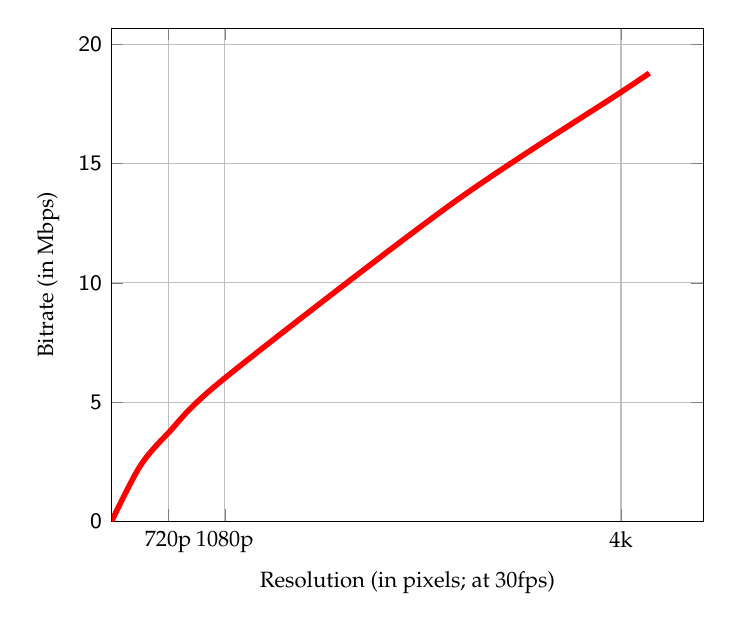
\begin{tikzpicture} %[>=latex]
\begin{axis}[
width=0.75\textwidth,
%line width=2,
%symbolic x coords={2012, 2013, 2014, 2015, 2016},
xtick={2,4,18},
xticklabels={720p,1080p,4k},
%minor xtick={0,1,...,18},
grid=both,
ymin=0,
xmin=0,
xlabel=Resolution (in pixels; at 30fps),
ylabel=Bitrate (in Mbps),
%enlarge x limits=0.1,
%xticklabel style={text width=0.2\textwidth,align=flush left},
]
\addplot[line width=2pt,smooth,color=red] coordinates {
	(0,0)
	(1,2.300)
	(2,3.700)
	%(3,5050)
	(4,6.006)
	(12,13.300)
	(18,18.000)
	(19,18.800)
};
%\draw[red] plot [smooth] coordinates {(0 0) (2,3700) (4,6006) (18,18000)};
\end{axis}
\end{tikzpicture}
	\caption{Bandwidth required for delivering various videos.}\label{fig:bitrate-resolution}
\end{figure}

To put this in perspective, let's look at the coming explosion in demand for network throughput. With the rapid progress of low-power wireless communications and the evolution of micro-sensors, the not-really-new concept of IoT begins to touch ground in novel fields like smart wearables, smart agriculture, smart homes, smart buildings, smart environments, smart cities, smart transportation, smart enterprises and smart hospitality. It is an undoubted trend that there will be an exponentially growing number of devices connecting to the Internet. 
In 2011, Cisco predicted that there would be 25 billion devices connected to the Internet by 2015 and 50 billion by 2020 \cite{evans2011internet}. 

Just imagine if these devices continually send 1K total-sized \texttt{HeartBeat} messages to the cloud in 1-second intervals. 
What kind of pressure will this put on backbone networks and cloud services in general? What challenges will network engineers face in coming years? And what new solutions will emerge? 

These challenges have forced the emergence of fog computing, a fairly new paradigm which basically moves some elements of Cloud Computing closer to the end users, especially in a machine-to-machine (M2M), collaborative platform; these elements include compute, storage, and networking devices \cite{Bonomi:2012:Fog:IoT}. 

Pear Limited, hereinafter referred to as ``Pear'', is an innovative start-up company that originated at the \emph{Foggy University}\footnote{It is a homophone of HKUST in Cantonese, because people in Hong Kong call it ``Foh Gei Dai Hok''; ``Foh Gei'' sounds like ``Foggy'' and means ``Science and Technology'', while ``Dai Hok'' means ``University''. Interestingly, every spring the HKUST campus is rather foggy because of its proximity to the sea. This fact makes the university live up to its ``Foggy'' nickname.} campus and mainly focuses on implementing fog computing technology from concept to reality. The business idea leverages future technological trends to meet real needs. 

Research on fog computing is still in its very early stages. On 19 November 2015, ARM, Cisco, Dell, Intel, Microsoft and Princeton University formed the OpenFog Consortium. It plans to set up seven different working groups aiming at solving problems in fog computing, but so far it has only published one architectural white paper\footnote{\url{https://github.com/OpenFog/white-papers/tree/master/Architecture}}. Therefore, Pear is neither required nor able to address all aspects of fog computing. Pear will first follow, implement, and practise a specific category of fog --- a relatively ``stable'' kind of fog, serving in-between the Clouds and the clients. It hopes it can get a foothold in this new market before the rules are established and before too many giant players join the game.

From one angle, Pear Fog is a descending cloud --- a pool of compute, networking and storage resources across the core through to the edge of the Internet. From another point of view, Pear Fog is a new and improved powerful peer-to-peer (P2P) system incorporated within a crowd-sourced paradigm, providing Infrastructure as a Service (IaaS), Platform as a Service (PaaS), or Software as a Service (SaaS) in a ``Uber''-like way. 
In addition, Pear Fog is compatible with and complementary to existing clouds. One of its goals is to serve as a coordinator of Cloud-Fog coordinators. 

We are implementing and operating a business-friendly subset of fog with crowdsourcing that helps fog demanders ({\em e.g.} some giant CPs and CDNs) cut their costs and provide better services to their end-users. Hereinto, the contributors ({\em i.e.} miners or fog node suppliers, including some of the end-users) can pair with Pear to form a pool of computational resources. 
Pear schedules the resources to process business tasks and rebate a portion of its profits to the contributors accordingly. The form of the awards can be the PRCToken (PearCoin Token), or a token issued by any of Pear's certificated business partners. 

To provide stable and sufficient fog services, Pear has to source and distribute a large number of fog devices powered by Pear's software, and it has several strategies to do so. %as well as to choose what and how to do carefully. 

This paper documents the following three contributions:
\begin{itemize}
	\item It presents a thorough survey of related fields along the pathway from the early days of networking to the Cloud to the Fog. 
	\item It proposes several effective approaches to offer fog services, in terms of software framework, network design, use cases, {\em etc.}
	\item It describes approaches to scale up the fog network, actualise the technologies, and from some mutually beneficial alliances to get off the ground and survive as a viable business in a cutthroat market. 
\end{itemize} 

We present an in-depth historical analysis of related areas. From the rises and falls of different technologies, as well as the ups and downs of different concepts, we share illuminating lessons. From these lessons, we summarise the key points and identify the best practices.   
The lessons stated in Chapter~\ref{sec-his-analysis} have inspired our decisions. 

We have decided to implement a business-friendly subset of fog first. We then provide further details on what we have chosen to do. Using analogy reasoning, we have arrived at a resolution to initially focus on single critical endeavour: implementing a multi-functional WebRTC gateway in C language. To make this business feasible, we need a stable hardware carrier with sufficient storage. We further analyse the types of fog resources and their dominant battlefields, and we generalise all the crowdsourcing fog services' model. We also analyse where fog will serve better than cloud, especially for content delivery. Finally we conclude by three medium-term projects. Thus, Chapter~\ref{sec-decisions} comes why, what and how we will develop our software and hardware products. 

To create a sustainable business, we carefully consider various product, price, place, promotion, partnership, and funding and financial plans. These are presented in Chapter~\ref{chp-biz-analysis}. 

\chapter{Business Analysis}\label{sec-biz-analysis}
In this chapter, we analyse our product, services and the market, and discuss our business decisions and plans. 

\section{Value Proposition}
The current value proposition of Pear is: to catalyse the sharing economy in computing. Pear works on precisely scheduling idle computing resources and bandwidth to match the demand/supply of all relevant parties through the Internet. We are learning from Uber, trying to involve more players to share and achieve multi-wins without destroying the current ecosystem. As there would be a number of services multiplexed on Pear's fog resources pool, it is infeasible to analyse them one-by-one. Here we only take Pear's Fog CDN service as an example. The changes of the industry chain can be illustrated as shown in Figure~\ref{fig:eco-sys-change}.
\begin{figure}[ht]
	\centering
	\includegraphics[width=.66\textwidth]{figure/biz/eco-system-change.png}
	\caption{Ecosystem change before and after Pear comes in.} \label{fig:eco-sys-change}
\end{figure}

The value proposition also illustrates the main reason why Pear is called ``Pear''. In ``The Three-Character Classic'' or ``San Zi Jing'', one of the most famous Chinese classic texts, an entire story is condensed into these twelve Chinese characters, means ``Aged four years, Rong proffered pears. Bear in mind, fraternally be kind''. The story mainly appreciates the then 4-year-old boy's virtue of being willing to share big pears to his elder and younger brothers. We extract the sharing spirit from this classic and find a better way to explain it with the success stories of Uber and Airbnb. Besides trying to make a profit, Pear is struggling to provide the best technical and economic means of P2P Internet sharing and to promote the concept of sharing resources for win-win situations via Fog Computing. 
\section{Services Offered}
Based on the concept and infrastructure of Fog Computing, Pear has the ambition of running hundreds of services that practise the philosophy of sharing economy. However, Pear is a company which surely needs revenue and profit in order to provide services consistently over time and grow to the next level. Thus, Pear is initially focusing on a few main services: 
\begin{enumerate}
	\item Fog media coding service;
	\item Fog CDN for live streaming and VoD (Video on Demand), aka Fog VDN;
	\item Fog VPN (virtual private network);
	\item Fog email delivery service;
	\item Fog computing for IoT.
\end{enumerate}

\section{Revenue Streams}
Pear is a technology-driven start-up company, with limited financial resources. The primary revenue during the beginning years will be generated from a business-to-business (B2B) model. Pear is responsible for developing customised fog service platforms for business partners and will charge them appropriate prices that help them save costs and/or generate more revenue. 

Take Pear's Fog CDN service as an example: CPs currently obtain traditional CDN services, which are mainly charged according to peak bandwidth consumed and which typically range from HKD~$30,000$ to $100,000$/Gbps/Month. For Pear's Fog CDN service, the price charged will be within HKD~$10,000$ to $15,000$/Gbps/Month. Pear would invest part of the revenue into regularly scaling up the network infrastructure in order to build a stronger Fog CDN offering more bandwidth and better usability. 

\begin{figure}[ht]
	\centering
	\includegraphics[width=.80\textwidth]{figure/biz/revenue_stream.png}
	\caption{Proposed revenue streams for Pear Fog's VDN service.} \label{fig:vdn-revenue-stream}
\end{figure}

\section{Distinctivenesses, Challenges and Risk Factors}
The brief introductions to Pear's technology and business have provided a rough picture of what Pear is, what it is doing and why it is doing it. Nevertheless, knowing how it works does not mean anyone can easily bring it into a real competitive market. Conversely, for projects like Pear's Fog VDN, the clearer people know about the details, the more likely they would realise that there is a solid barrier to success. 

The most difficult task throughout the development of Pear's Fog CDN platform has been to elegantly build the framework with pure C language. The platform interfaces with the front-end media control using HTML5 and JavaScript, with the back-end schedulers and servers using C++ and FastCGI, and with the embedded system programs using C and assembly. That is already beyond an ordinary full-stack engineer's range.

Howbeit, Pear can do even more. A traditional programmer would probably not be qualified to lead this project, because the Fog CDN platform also requires expert knowledge in streaming and network protocols, like WebRTC, HLS and MPEG-DASH, as well as various open P2P protocols. Even inside IT Giants, it is hard to find such guys with such versatile skills. Fortunately, Pear's three technology co-founders' backgrounds cover all these special criteria. Pear Fog is a demanding project in terms of hardware and software engineering, and it is also highly correlated to the newest Internet technology, which sets barriers for potential competitors. Only a special ops hardware and software team could try to do what Pear is doing.

In spite of all Pear's human capital, it does face some challenges and associated risks: 
\begin{enumerate}
	\item Pear does not yet have much capital investment. This shortage of funding could hinder Pear from scaling up rapidly. 
	\item Pear is overstretched with human capital. The team will have to work very hard and smart to achieve its goals in the given time frame.
	\item Pear still lacks its own market resources. It must initially solely rely on its partners, such as router vendors and CPs, and Pear knows it is a little bit over-reliant upon them. 
	\item The trial-test-and-pay nature of B2B businesses would make the revenue come relatively late. 
\end{enumerate}

Nevertheless, Pear's risk factors should also help Pear to work hard and work smart. We are young, eager and confident that Pear will grow much stronger soon. 
This is based on our working experience, input from experts and relationships in the CDN field and elsewhere that should encourage win-win cooperation.

\section{Product and Marketing Plan}
Among all the services we are offering, Fog CDN is Pear's featured product. It is a huge system, and we plan to steadily build it step by step, firmly. We believe the Fog CDN market will eventually capture people's attention. We also expect the Fog CDN to be the ever first successful product based on fog computing technologies. 

\subsection{Market Analysis}
Pear is an innovator in the CDN market. We are not able to tell whether our Fog CDN will completely replace the traditional CDN's role, but we aim to make it step gently into the traditional CDN market and gradually capture more and more market share until the two coexist and complement one another for a relatively long time in the future. 

\subsubsection{Target Customers}
In Pear's B2B Model, the targeted customers mainly refer to the CPs and traditional CDN service providers. 

Because of the inherent advantages of the background of one of the co-founders, Pear has a close relationship with the biggest video content provider in mainland China: Tencent Video. Pear's initial marketing efforts will focus on Mainland China since it is the largest market in the world and most of the co-founders are Chinese. 
Pear now is helping a new CDN provider to build a video cloud platform which implements part of Pear's Fog CDN technology aiming to help deliver the 4k video smoothly, and with a reasonable cost.

As user generated content (UGC) becomes more popular on the Internet, Pear expects to see some new types of CPs that leverage UGC business, such as BiliBili.com and ACfun.tv. Pear will also target them as customers in the first stage.

Due to the versatile Fog CDN infrastructure, as Pear grows, we can reuse this network to build the Fog VPN service with a high degree of usability. Pear plans to present consumers with the Fog VPN service in the second stage after the B2B business is proven to be viable.

\subsubsection{Market Characteristics and Trends}
From a commercial CDN market survey report, we can see that the Total Addressable Market (TAM) of the commercial CDN is increasing at a phenomenal rate, especially in China, see Figure~\ref{fig:CN-CDN-TAM}. 

\begin{figure}[ht]
	\centering
	\begin{center}
		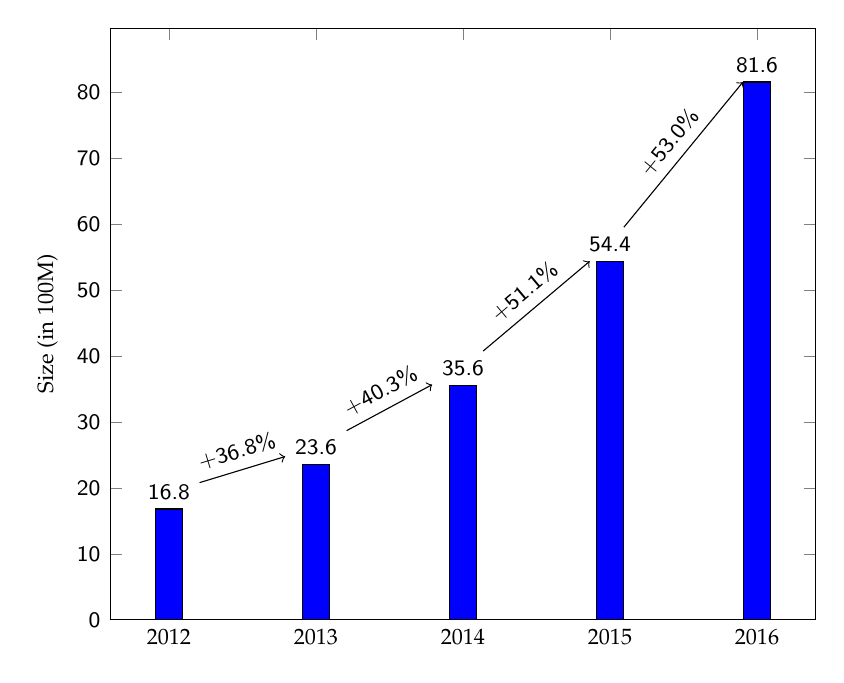
\begin{tikzpicture} %[>=latex]
		\begin{axis}[
		height=0.75\textwidth,
		symbolic x coords={2012, 2013, 2014, 2015, 2016},
		xtick=data,
		ymin=0,
		ylabel=Size (in 100M),
		enlarge x limits=0.1,
		%xticklabel style={text width=0.2\textwidth,align=flush left},
		]
		\addplot[ybar, axis on top, fill=blue] coordinates {
			(2012, 16.8)
			(2013, 23.6)
			(2014, 35.6)
			(2015, 54.4)
			(2016, 81.6)
		};
		\node (n2)[above] at (axis cs:  2012,  16.8) {$16.8$};
		\node (n3)[above] at (axis cs:  2013,  23.6) {$23.6$};
		\node (n4)[above] at (axis cs:  2014,  35.6) {$35.6$};
		\node (n5)[above] at (axis cs:  2015,  54.4) {$54.4$};
		\node (n6)[above] at (axis cs:  2016,  81.6) {$81.6$};
		\draw [->] (n2) -- (n3) node [midway, above, sloped] (tn1) {$+36.8\%$};
		\draw [->] (n3) -- (n4) node [midway, above, sloped] (tn2) {$+40.3\%$};
		\draw [->] (n4) -- (n5) node [midway, above, sloped] (tn3) {$+51.1\%$};
		\draw [->] (n5) -- (n6) node [midway, above, sloped] (tn4) {$+53.0\%$};
		\end{axis}
		\end{tikzpicture}
	\end{center}
	\caption{TMM of China Market.}\label{fig:CN-CDN-TAM}
\end{figure}

\begin{figure}[ht]
	\centering
	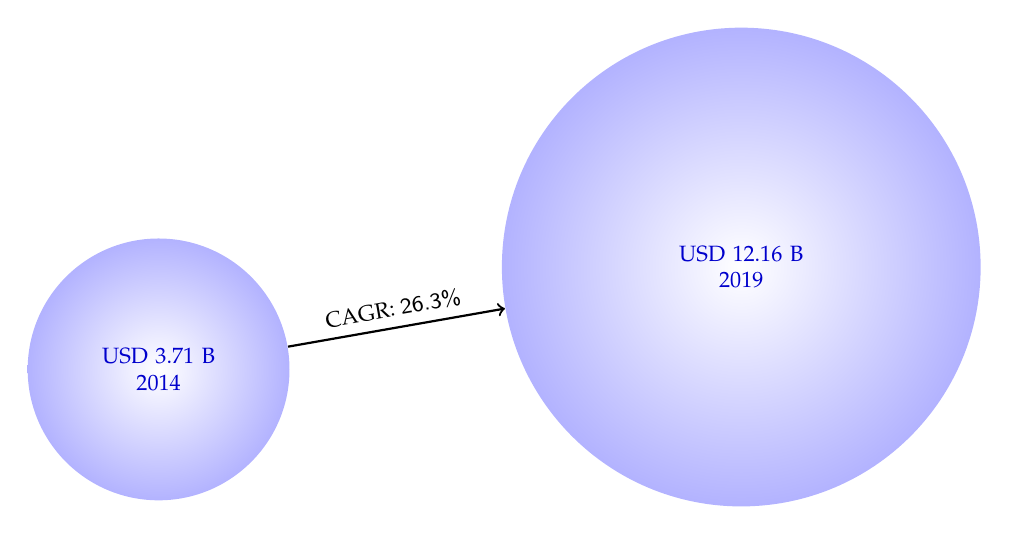
\begin{tikzpicture}
	\node(c1) [circle,shading=radial,outer color=blue!30,inner color=white,
	minimum width=1.855cm,align=center,text width=3cm] at (0.1,3.3) {\textcolor{blue!80!black}{USD 3.71 B\\ 2014}};
	\node(c2) [circle,shading=radial,outer color=blue!30,inner color=white,
	minimum width=6.08cm,align=center,text width=3cm] at (7.5,4.6) {\textcolor{blue!80!black}{USD 12.16 B\\ 2019}};
	\draw [->, thick] (c1) -- (c2) node [midway, above, sloped] (c1c2) {CAGR: $26.3\%$};;
	\end{tikzpicture}
	\caption{Cisco's world commercial CDN TAM growth expectations from 2014 to 2019.}\label{fig:World-CDN-TAM}
\end{figure}

According to a prediction by iResearch, the TAM of China's commercial CDN is expected to reach RMB 8.16 billion in 2016 with an annually increase at about 53\%. 
In fact, we have witnessed that all previous CDN market size predictions were eventually proven to be far behind the real growth. For example, in a Cisco white paper published in 2014, the world's commercial CDN TAM in 2012 was predicted to reach USD 12.16 billion at a CAGR of 26.3\% as depicted in Figure~\ref{fig:World-CDN-TAM}, while a report\footnote{\url{http://www.researchandmarkets.com/research/8vnkvv/mobile_cdn_market}} issued in 2015 suggested that the mobile CDN market alone will grow from USD 2.11 billion in 2015 to USD 13.40 billion by 2020, at a CAGR of 44.7\%. 

The fact is telling us: data traffic demand tends to run far over the commercial CDN capacity. Moreover, the gap between demand and supply is becoming wider and wider. When we compare China's market and the World's, we find that commercial CDN only serves 8-10\% of total Internet data traffic in China, while in the US, commercial CDN has already been serving around 50\% Internet data traffic. This is another reason why Pear is focusing on the China market in the first stage.

Apart from that, we expect that the demand for commercial CDN will last for long, so we are sufficiently confident with its market, even in the global depression. This is because commercial CDN mainly serves online video, games and related entertainment industries that are expected to perform very well regardless of the economic outlook. History shows that Broadway and Hollywood thrived during the Great Depression, so unless there is a war or global cataclysm, we expect similar favourable conditions in the CDN market. 

\subsubsection{Revenue Potential}\label{revenue-potential}
During stage one, we have a simple method to estimate the revenue of this business:
Assume a CP needs 8Tbps bandwidth for delivering its video content, 1\% of its traffic is 80Gbps. For the general case of CDN bandwidth price, HKD~$30,000$/Gbps/Month, 1\% of his traffic will cost HKD~$2.4$ million. For our Fog CDN, we need only around $8,000$ signed smart routers to share their idle uploading peak bandwidth less than 10Mbps. With our pricing strategy, we will only charge this CP HKD~$1.2$ million as the service price. In this case, the CP will save HKD~$1.2$ million to and be able to purchase the broadcasting rights of more video content, and we will also have the flexibility to manage our income. For example, we could return HKD~$600$k cash or equivalent VIP memberships to the $8,000$ signed users, and retain left HKD~$600$k as profit.

The above scenario only shows the starting case of taking 1\% of this CP's data traffic. The business is clearly scalable, because if we have more signed home/business routers and idle bandwidth, we will be able to take more traffic volume. Above all, there is only one CP for this illustrative example. In reality, we can provide this Fog CDN to multiple CPs with both a sweet price and good quality. Our target is to serve as many CPs as possible within our capability. 

\subsection{Product \& Service Plan}
Pear has divided its product and service marketing plan into three stages, as describes in Table~\ref{tb:product-market-plan}. 
\begin{table}[htb]
	\centering
	\caption{Pear's first three stages of its product and service and marketing plan.}\label{tb:product-market-plan}
	\footnotesize
	\begin{tabular}{p{0.11\linewidth}p{0.28\linewidth}p{0.28\linewidth}p{0.28\linewidth}}  
		\toprule
		Stage &    Stage 1    & Stage 2 & Stage 3 \\
		\midrule 
		Time & Year 0-1.5 & Year 1.5-2 & Year 2+ \\
		End-users & Low awareness of Pear's Fog Computing \& sharing economy philosophy & High awareness of Pear's services & Actively install Pear to their own devices to join Pear's world\\
		Cooperating Firms & {Pear has no user base at this stage. We need to cooperate with large user-base companies to build up the Pear Virtual Network: HW: MeegoPad, AllWinner, Huawei, Intel; CP: Tencent Video, imeme.tv; Pear's own device: in design} & {Pear will have built up a broad-range network. Cooperating firms (mostly CPs) gradually become Pear's customers} & {Pear will not be depending solely on the end-user base of cooperating companies}\\
		Target Customers & {Testing with cooperated firms; small or medium CPs} & {Large CPs, especially cooperating companies} &    All web CPs\\    
		\bottomrule
	\end{tabular}
\end{table}

\subsubsection{R\&D Milestones}
Pear plans to launch the Fog email delivery and Fog CDN services at the same time since quite a number of elements overlap. It is highly efficient to reuse the resources while achieving multiple targets, although the email delivery source may not be used as thoroughly as the Fog CDN. The detailed milestones are shown in Table~\ref{tb:rd_milestone}. 
\begin{table}
	\centering
	\caption{Pear's R\&D Milestones}\label{tb:rd_milestone}
	\small
	\begin{tabular}[t]{ccp{0.68\linewidth}}  
		\toprule
		\multicolumn{2}{c}{Period} \\
		\cmidrule(r){1-2}
		From & To & {\textsc{~~~~~~~~~~}Description}\\
		\midrule
		01/02/2016 & 01/03/2016  & {1. Basically finish the protocol, API, and architecture designs for Pear's fog computing system.\newline 2. Establish one or two partnerships in which we help partners solve cost optimisation problems and hopefully gain some referrals and/or more attractive contracts.}\\
		01/03/2016 & 01/09/2016    & {Implement Pear's fog computing protocols on the firmware of Pear's routers and/or IPTV set-top boxes (all-in-one devices).}\\
		01/09/2016 & 01/10/2016 & {1. Enable Pear's fog computing system on the live streaming platform(s) of partner(s) of Pear.\newline 2. Provide open source versions of some components of Pear's fog computing project under MIT, Apache, BSD or GPL license(s), and at the same time maintain a commercial version.\newline 3. Create real impacts in the corresponding industry, especially the open source communities.}\\
		01/10/2016 & 01/02/2017 & {1. Complete the project developed for Partner 1 (Probably ``Fog'' email delivery and HD video transmission).\newline 2. Complete the project developed for Partner 2 (``Fog'' live streaming service platform).}\\
		01/02/2017 & 01/12/2017    & {Launch and complete the project developed for Partner 3 (“Fog” Multimedia CDN)}\\
		\bottomrule
	\end{tabular}
\end{table}

\subsection{Marketing and Sales Strategy}
We have carefully thought through the four Ps of marketing: product, promotion, place, and pricing. Our strategies for each of these are introduced below. 

\subsubsection{Product Strategy}
Pear's Fog CDN service is designed to run like a duet: it serves both the CPs \& ISPs and the end-users simultaneously, like a precise driving gear powering its driven counterparts automatically.

Pear is already prepared to cooperate with ISPs who have a large user base but are weak in cloud data centres (such as China Mobile) and hardware vendors (such as Huawei). Through this fundamental work, the end-users will enjoy:
\begin{enumerate}
	\item Faster Internet access and a better video streaming experience;
	\item Remote control, monitoring and management for the signed smart devices;
	\item Real cash/coupons or VIP service as a reward for sharing their idle bandwidth.
\end{enumerate}

Pear is ready to provide high-quality CDN services, initially mainly for online video CPs, promising to reduce operating costs significantly. For these wise content providers, they can enjoy: 
\begin{enumerate}
	\item Better streaming quality and transmission efficiency of CDN services;
	\item Better geographical access coverage;
	\item Significantly lower content delivery cost;
	\item ``Flash-crowd'' and ``bottle-neck'' headaches minimisation.    
\end{enumerate}

\subsubsection{Promotion Strategy}
Pear plans to use common channels, like social media and mass media, for public awareness.
At the same time, Pear is leveraging media resources of device vendors (agreed), Intel (agreed), Tencent, and JD.com crowd-funding for promoting the fog computing devices and services. There are three main methods Pear is going to use for promotion in B2C model as illustrated in Figure~\ref{fig:promotion-strategy}.  
\begin{figure}[ht]
	\centering
	\includegraphics[width=.80\textwidth]{figure/biz/promotion_strategy.png}
	\caption{Promotion strategies for Pear's B2C Model.} \label{fig:promotion-strategy}
\end{figure}
\begin{enumerate}
	\item Cash rewards or interest-free instalments as incentives. Pear even can deliver the smart routers for free to end-users who sign an agreement to stay online 24/7 to provide bandwidth for the Pear Fog, thus helping the network accommodate more traffic or content delivery volume.
	\item CP VIP memberships to leverage activities or direct exchange with end-users, so they will contribute bandwidth to support more network traffic.
	\item Cooperation with the ISPs and/or telecom operators, such as China Mobile. Pear will be able to provide them with the scaled end-users' contributed traffic volume through cellular phones' data networks.
\end{enumerate}

\subsubsection{Place and Channel Strategy}
Initially, Pear must partner with vendor companies to bundle Fog services with their smart devices, such as routers and TV boxes, as well as mini PCs to establish a wider user base among the general public.

For most of the initial stage, Pear will not face consumers directly, so Pear must focus on its B2B channel to first help vendors with their bandwidth needs. However, at a later stage, Pear would pay much more attention to its B2C channel, which is related to the life and death of Pear in the long run. Otherwise, vendors would eventually develop their own in-house fog platforms and go around us, thus leaving us without work to do. 

Facing customers will not only help with our longevity, but it will also help us better understand their needs and wants and serve them directly. Thus, Pear will pay full attention to all possible channels that could reach the consumers.
% Only when we could face with customers directly, we have the initiative of development and going concern. So Pear would pay full attention to all possible channels that could reach the consumers.

\subsubsection{Pricing Strategy}
For Pear's Fog CDN service, its price will initially be about HKD~$12,000-15,000$/Gbps/month. This price is about 40\% of the currently cheapest traditional CDN competitors in Mainland China. Pear is also considering other flexible pricing schemes for different scenarios, {\em e.g.}, by total traffic/size of data, by user base, by coverage of outlying regions and edge ISPs, and by the load shifting effect. Pear's aim is to always be to provide equivalent or better quality CDN services at less than half of the original pure-traditional CDN price. 

\subsection{Competition}
Pear is an innovator in the relatively mature traditional CDN market. We will face challenges from existing giants who are also considering Fog CDN as well as from the other innovators with similar Fog CDN services. On the other hand, these competitors could also be Pear's customers and partners. Thus, Pear keeps an open mind to the competition and expects all interested communities and individuals to join in the fog computing world to explore and contribute. One proof of this open-mindedness is that Pear has already kept and will always keep all wheel-like core components open source. This is similar to the early Microsoft model of allowing its software (MS-DOS) to be freely copied all over the world, which gave it a clear victory over IBM's PC-DOS, which became the standard for most PCs in the 1980s. IBM did not foresee the rampant of ``file sharing'' of PC retailers in countries outside the US, nor did it expect Bill Gate's tiny start-up to actually gain so much from it. This was all thanks to a non-exclusive agreement that the tiny start-up signed with the computing giant in 1980 \cite{ms-ibm-dos}. 

\subsubsection{Traditional CDN Competitors in Mainland China}
In China, there are two outstanding traditional CDN giants to whom Pear is paying attention: ChinaNetCenter and ChinaCache.

In 2014, ChinaNetCenter had a market share of about 43\%, and ChinaCache about 37\%. In 2015, ChinaNetCenter had revenue over RMB 2 billion, with a market capitalization at around RMB 30 billion, and ChinaCache had a market capitalization at USD 185 million while its revenue was around USD 220 million. 

Among the two CDN giants, ChinaCache is more willing to access new technology, since it has recently signed a cooperation contract with HiWiFi Router and Youku LuYouBao. Pear looks upon ChinaCache as one of the biggest competitors, and sincerely admires its strategy as well as executive power. On the contrary, Pear looks forward to potential cooperation opportunities with ChinaNetCenter. 

\subsubsection{New-born Competitors in China Mainland}
From 2015 till now, Pear only has two new competitors in the Fog CDN market: Xunlei (Thunder) XYCDN\footnote{\url{http://www.xycdn.com/}} and Youku LuYouBao\footnote{\url{http://yj.youku.com/luyou}}.

Xunlei originally is a download manager and Peer-to-peer software developed by Thunder Networking Technologies, supporting HTTP, FTP, eDonkey, and BitTorrent protocols. As of 2010, it was the most commonly used BitTorrent client in the world. On 24 June 2014, it went public on the Nasdaq Stock Exchange, raising 88 million USD. Xunlei's advantage concentrates on file downloading techniques which are essential for Fog CDN. Moreover, now Xunlei has just adjusted their strategic direction to ``crowd-sourced CDN''. Their CDN, called XYCDN, is their featured product right now. The product is still naive but has efficient iterations. Xunlei has just announced their 2nd Generation ZhuanQianBao miner: a low-cost mini server which when plugged into users' home routers, is ready for sharing not only idle bandwidth but also storage.

Youku Tudou Inc. is one of China's biggest video CPs, having a market capitalization of over USD 5 billion. It is aggressively investing in innovative technology that enhances its services while reduces its cost. Recently, it was reported that Youku had sold over 500k 1st generation LuYouBao intelligent network terminals in 2015. Different from the Xunlei ZhuanQianBao miner, LuYouBao is a smart router with full functions. Youku LuYouBao signed a co-development contract with ChinaCache in 2015, so Pear sees these joined forces as great competitors. 

\subsubsection{New-born Competitors outside of the Greater China}
Unlike the Chinese competitors who focus on CDN hardware, Pear's international competitors are leading the software and platform design for the P2P CDN industry.

One of the competitors is named Peer5. Established in 2012, Peer5 is a CDN provider that leverages WebRTC (see Appendix B) to improve content delivery with the assistance of P2P technologies. Peer5's offerings include a live streaming CDN, a radio streaming CDN, a big object downloader, a VoD CDN and image loading service. Peer5 has already received angel investment and has over ten staff working full-time. The idea of leveraging WebRTC protocol coincides with Pear's Fog CDN R\&D plan. This fact gives Pear confidence, and Pear appreciates Peer5's courage to be the first mover to help the P2P CDN industry get a second wind. Currently, Peer5 is not doing much in China, but if Pear expands outsides of China, especially in western countries, Peer5 is likely to be a competitor.

\subsubsection{Pear's Comparative Advantages}
\begin{itemize}
	\item Pear's comparative advantages over traditional competitors\\
	Although a traditional CDN is easy to schedule in the initial stage, two critical shortcomings lie in front of a traditional CDN company when it is going to scale up. One is the cost. Even for the biggest traditional CDN provider with sophisticated cost control, the bandwidth's price is still two to three times as much as that of the Pear's Fog CDN. The other is the geographic limitation. Since traditional CDN deployment requires data centres, the outlying regions and edge ISPs typically meet trouble to set up CDN servers.
	
	On the contrary, because end-users' smart devices are working as distributed CDN servers, Pear's Fog CDN servers can instantly work anywhere Internet users exist. Pear will never face the same problems as its traditional CDN competitors do when scaling up or expanding geographically. This is similar to the advantage Microsoft had over  IBM in the 1980s. 
	
	\item Pear's comparative advantages over new-born competitors in China\\
	The new-born Chinese competitors all have one problem in common: neglecting the system architecture design at the beginning. It is understandable that companies have pressure to bring in income as soon as possible. However, in Xunlei XYCDN's case, stuffing the miner with outdated HTTP server techniques along with proprietary protocols as a crowd-sourced CDN server, has created hidden risks in case other competitors prove that the WebRTC protocol is overwhelmingly useful for Fog services, on which Pear is now working. With old and proprietary (and exclusive) protocols and modules, Xunlei's CDN service is completely Web-unfriendly: the end-users need to install apps or clients; the served CPs need to modify their source code to call Xunlei's services as well. Thus, they are not user and CP transparent. So these issues will be a stumbling block to Xunlei in the future if they cannot realise it and rectify it in time. 
	
	The differences between Xunlei's hardware and Pear's hardware are briefly summarised in Figure~\ref{fig:hw-comp-xunlei}.
	\begin{figure}[ht]
		\centering
		\includegraphics[width=.88\textwidth]{figure/biz/hw_comp_xunlei.png}
		\caption{Comparison between Xunlei's and Pear's hardware.} \label{fig:hw-comp-xunlei}
	\end{figure}
	
	\item Pear's comparative advantages over new-born global competitors\\
	When we consider competitors like Peer5, it is rather respectful and admirable to have such a strong R\&D team fighting on the frontier. WebRTC is an advanced, future-oriented protocol for communication between any browsers. It can easily enable P2P communication and maintain the web-friendliness at the same time. That is why Pear shares a similar concept for implementing WebRTC protocol as the infrastructure of Pear's Fog CDN. 
	
	However, there is one problem that Peer5 may have considered but has no solutions for right now. Peer5's CDN service is based on the web browsers on desktop PCs, whose behaviour is unpredictable because the user behaviour behind them is random. In large-scale commercialised services, Peer5's performance will be affected, and they need to find a way to try to keep most of the nodes always working online. Bur it is hard, because they have no enough monetary incentive to encourage the end-users to keep their PCs and browsers running 24/7.
	
	Pear has chosen another approach --- a deliberate method to ensure each nodes' stability as a Fog CDN server. We are embedding the WebRTC protocol directly into routers with pure C language.
	Experienced engineers will know the difficulties on the way to success, and we are determined to achieve success on the way. We are now working to overcome the highest hurdles for popularising the Fog computing technology into reality. We are also seeking talented engineers and professionals to join us. 
	
	Pear has another inherent advantage: geographic proximity. Pear is based in Hong Kong and Shenzhen, which enables us to develop connections with various router, TV-box and mini PC vendors in these two thriving cities. This makes it easy to cooperate and receive technical support more easily, compared with Peer5 or other competitors outside China.
	
	\item Pear's comparative advantages over other start-ups by fresh graduates\\
	Pear's founders have an unusual background. The three of them combined have a dozen years of professional experience in the networking field, and two of them are currently pursuing postgraduate degrees at HKUST in the prestigious TLE program. Combining their connections and resources from the industry with their advanced research work, they have put together a dream team for Fog CDN services and smart router innovation. They are not merely IT guys. 
	
	With technical experience, not are they academics with lots of conceptual knowledge but no practical industry experience. They have the best of both worlds.
	%Pear is a little bit unusual for its background. Three of the co-founders have years of working experience, and two of them are back to university although they already have achievements in their career. They brought back the connections and resources from the industry and through the research work in HKUST, they polished their entrepreneurship ideas. Finally, with endless passions, these guys started the new story at the ever highest point, and this is how pear begins.
	
	%Moreover, also this is the one difference between Pear and the other start-ups mainly composed of PhDs and professors who have never or rarely been deeply involved in the real industry. 
\end{itemize}
In summary, Table~\ref{tb:features-pearcompetitors}, Figure~\ref{fig:cost-performance-competitors} and Figure~\ref{fig:all-essences-advantage} provide comparisons of Pear with its primary competitors. 

\begin{table}[hb]
	\footnotesize
	\centering
	\caption{Features of Pear Fog VDN and its competitors}\label{tb:features-pearcompetitors}
	\begin{tabular}[t]{p{0.08\linewidth}p{0.05\linewidth}p{0.05\linewidth}p{0.06\linewidth}p{0.05\linewidth}p{0.25\linewidth}p{0.14\linewidth}p{0.10\linewidth}}  
		\toprule
		Product & Wi-Fi AP & Media CDN & Patented & Rebate profit to end-users & Price @ CP side & Coverage & Targeted Customer\\
		\midrule
		Pear & Yes & Yes & Yes & Yes & HKD~$12$K/Gbps/month & Worldwide\tablefootnote{We start with the Greater China and branch out in Asia; One Belt, One Road (OBOR) countries will also be target regions: they have 60\% of the world's population and way be happier with fog.} & Any CP\\
		Thunder XYCDN & No & Yes & No & Yes & CNY~$10$K/Gbps/month & China & Large CP\\
		ChinaNet-Center & No & Yes & No & No & CNY~$60$K+/Gbps/month    & Mainly China & Traditional Websites\\
		Akamai & No & Yes & Yes & No & Depends on service region,  generally expensive & Worldwide (except China) & Traditional Websites\\        
		\bottomrule
	\end{tabular}
\end{table}

\begin{figure}[ht]
	\centering
	\includegraphics[width=.8\textwidth]{figure/biz/cost-performance-competitors.png}
	\caption{Cost/Performance view on Pear and its competitors.} \label{fig:cost-performance-competitors}
\end{figure}

\begin{figure}[htb]
	\centering
	\includegraphics[width=.8\textwidth]{figure/biz/all-essences-advantage.png}
	\caption{Illustration of why Pear is ``tasty''.} \label{fig:all-essences-advantage}
\end{figure}

\subsubsection{Potential Competitors in Emerging Fields}
Potential competitors in emerging fields may be grouped into two categories: 
\begin{itemize}
	\item Cloud WebRTC Service Providers 
	\item IoT Fog Computing Service Providers
\end{itemize} 

The first group is characterised by products which are enabling mobile apps and web pages with real-time communication capabilities. They offer the web and mobile SDKs that connect to their cloud WebRTC services and charge business users based on total connections, sessions or bits. An example is Agora, founded by YY Live's co-founder and ex-CTO. Agora raised USD 25.9 million in its Series A and B investments in 2015. It then sponsored the world's most influential WebRTC conference and translated a WebRTC standard book to Chinese, which made it the most well-known WebRTC-specialised technology company in China. 

The second category is characterised by businesses that are bringing intelligence to the edge. FogHorn is a such example. It provides an edge software stack for industrial IoT that ingests the data from sensors and industrial devices onto a high-speed data bus and then executes user-defined analytics expressions on the data stream to gain insights and optimise the devices. ForHorn secured USD 12 million in Series A funding on 27 July 2016. 

Pear acknowledges strong competition from these competitors. However, viewed from another angle, the competition will help bring the WebRTC and Fog concepts to the industry. Pear's initial revenue source is expected to be from services to Cloud providers, while its own emphasis is the Fog. The Fog requires wide coverage by a huge amount of enabled nodes, while the Cloud only requires a simple ``one-click-enabling''. 

\subsection{Strategic Partners}
Before introducing Pear's strategic partners, it is necessary to have a full view of China's “CP+Vendor+CDN” ecosystem in Figure~\ref{fig:cp-vendor-cdn}.
\begin{figure}[ht]
	\centering
	\includegraphics[width=.75\textwidth]{figure/biz/cp-vendor-cdn.png}
	\caption{Rough view of power distribution in the ``CP+Vendor+CDN'' ecosystem.} \label{fig:cp-vendor-cdn}
\end{figure}

It is not surprising to see the ``BAT (Baidu-Alibaba-Tencent)'' allied pattern in the current market; after all, they are the only three dominant giants in China's IT industry. Right now, Pear has cooperation with Tencent. In the meantime, Pear is trying to be neutral to all CPs, since the quickest way to promote the Fog CDN service is to open it to everyone.

We can see that there still exist neutral or unallied formidable players in the industry, and Pear is aiming at prioritising cooperation with these participants, such as Huawei, Pear has already negotiated with Huawei and has reached an initial agreement on co-developing the APIs on top of Huawei Honour router's customised firmware. 

\subsubsection{Vendor Partners}
Pear Fog CDN edge programs are fundamentally designed to be cross-platform and can be installed on every smart device with Windows or Linux OS, {\em e.g.} home routers, TV boxes, PCs, self-hosted servers and even cellular phones. To achieve the optimal result, we chose routers as the best candidates mainly because:
\begin{enumerate}
	\item they can ensure a high probability of 24/7 online connectivity;
	\item they have a good chance of obtaining public IP addresses, which reduces of at least one layer of NAT traversal, which can mean much better accessibility. 
\end{enumerate}

Pear will not have hardware manufacturing capabilities until January 2017, so Pear has acquired several hardware partners for developing and testing Pear's Fog CDN services.

\begin{itemize}
	\item NetGear Hong Kong\\
	NetGear is a US-headquartered global networking company that specialised in producing high-end routers for retail and business markets. NetGear Hong Kong has offered Pear and RADICA four Nighthawk R8000 and one R7000 routers (see Figure~\ref{fig:netgear-r7000-r8000}) for developing and testing the Fog email delivery project. RADICA also proposed to deliver a few thousands of routers in Hong Kong and Taiwan to launch a fog computing platform. 
	\begin{figure}[ht]
		\centering
		\includegraphics[width=.7\textwidth]{figure/biz/netgear-r7000-r8000.png}
		\caption{NetGear Nighthawk R7000 and R8000 Wi-Fi Routers.} \label{fig:netgear-r7000-r8000}
	\end{figure}
	\item Huawei Honor\\
	Huawei Honor has independent R\&D and marketing teams. In 2015, they sold over two million ``Honor Routers''. The Huawei Honor R\&D team has agreed to open their proprietary APIs to Pear to enable Pear's fog computing services. However, after some small trials, Pear engineers found Honor's VM environment is currently not friendly to native C program development. The porting work has been put on hold for one year. 
	\item QNAP\\
	Headquartered in Taiwan, QNAP is the 2nd largest global NAS vendor. Intrigued by Pear's Sharing Fog Computing concepts, QNAP had a meeting with Pear in Shenzhen in early autumn 2016. QNAP expects to see when Pear schedules the computational resources of 5,000,000+ QNAP devices (see example types in Figure~\ref{fig:qnap-x51}) worldwide and brings value added to the device owners. QNAP is willing to promote Pear's software with its own channels. After that meeting, QNAP offered Pear the latest SDK (called QDK) to make the development easier. A tentative plan is to beta test the software by January 2017 and launch the service by March 2017.
	\begin{figure}[ht]
		\centering
		\includegraphics[width=.7\textwidth]{figure/biz/QNAP_x51.jpg}
		\caption{QNAP x51 Series.} \label{fig:qnap-x51}
	\end{figure}
	\item MeegoPad\\
	MeeGoPad was the earliest vendors to offer its hardware for Pear's R\&D and testing. In fact, MeeGoPad is the biggest ODM \& OEM for Intel Compute Stick product line in China. They have promised to develop a customised carrier to run Pear's fog services. Pear is preparing the supporting software for the so-called \emph{Pear Stick} or \emph{Pear Sharing Box} at this moment. Beta testing is scheduled for January to March 2016, and Pear hopes to begin marketing it in April 2017 and shipping it to vendors and crowd-funding platforms in May 2017.
	\begin{figure}[ht]
		\centering
		\includegraphics[width=.7\textwidth]{figure/biz/huawei-honor-and-meego-stick.png}
		\caption{Other carriers of Pear Fog: Huawei Honor Router and MeeGopad Compute Stick.} \label{fig:huawei-honor-and-meego-stick}
	\end{figure}
\end{itemize}

\subsubsection{CDN Partners}
Shanghai Maichuang Network Technology Co., Ltd. (aka Tan14\footnote{\url{https://www.tan14.cn/}}) is a CDN start-up company with seemingly strong financial strength and based in Shanghai. They have admirably extensive connections with CPs, and their customers have already generated enough profit for scaling up and investing in R\&D. Currently, they have more than 80 CDN nodes distributed in Mainland China and Hong Kong as well as Taiwan.

Pear and Tan14 have reached a cooperation agreement to build an entirely new cloud \& fog integrated platform for live streaming by the end of 2016. Pear is responsible for architecture design and software implementation coordination, while Tan14 has promised the customers and the investment. Hopefully it will be a win-win partnership.

\subsubsection{CP \& SP Partners}

\begin{itemize}
	\item Tencent\\
	Tencent Video is one of the biggest online video content providers in Mainland China. It has a private CDN to support the growing bandwidth demands. However, as Figure~\ref{fig:tencent-youku-cost-growth} depicts, it is now facing a serious cost/revenue bottleneck. Tencent Video and Pear have also reached an agreement for scheduling and testing the Pear Fog CDN when Pear's active routers arrive at a certain number. As mentioned in Section~\ref{revenue-potential}, Tencent Video will immediately resolve their cost bottleneck once they are equipped with Pear's Fog CDN.
	Besides Tencent Video, Pear also has oral agreements with two other Tencent subsidiaries Qzone's and QQ Video Album's teams plan to schedule the video content delivery through Pear's Fog CDN when it is ready.
	\begin{figure}[ht]
		\centering
		\includegraphics[width=1.00\textwidth]{figure/biz/tencent-youku-cost-growth.png}
		\caption{Some CPs' cost growth rate.} \label{fig:tencent-youku-cost-growth}
	\end{figure}
	
	To summarise the partnership with Tencent: Pear has the chance to test the Fog CDN serving:
	\begin{enumerate}
		\item the largest online video platform in China (in terms of traffic); 
		\item the largest social networking service in China;
		\item and one of the largest photo album platforms in the world.
	\end{enumerate}
	
	\item RADICA\\
	RADICA Systems is an HKUST alumni-owned IT company based in Hong Kong. With 15 years of experience, RADICA has mainly helped Asia Pacific brands and enterprises to effectively perform direct marketing. Over 300 enterprises are now their customers. With the aid of Pear's fog computing platform, RADICA expects to be able to provide its current services at an astonishingly lower price so that they can hopefully increase their customer base.
	
	RADICA, Pear and NetGear are now jointly launching a ``fog email delivery'' project. Pear is responsible for the software and RADICA is responsible for the customers and technology support for the email servers'resources. Currently, the project is successful in the first stage; the prototype is working online. In the second stage after Autumn 2016, RADICA and Pear will start a large-scale test in a real commercial scenario. This fog email pushing project is critically important to Pear since it contributes to building the fundamental framework of Pear's fog computing network. Pear will save time in developing its Fog CDN and Fog VPN infrastructures thanks to this fog email pushing product. 
\end{itemize}

\subsection{Operating Plan}
\subsubsection{Hiring and Development Plan}
Pear plans to scale up to around 10-15 staff by mid-2017, including three owners. Details are in Table~\ref{tb:hiring-plan}. 
\begin{table}[ht]
	\centering
	\caption{Pear's Hiring Plan.}\label{tb:hiring-plan}
	\begin{tabular}[t]{llr}  
		\toprule
		Time (mm/yyyy) & Vacant Positions & Number on Plan\\
		\midrule
		09/2016    & Front-end Engineer &    1\\
		10/2016    & Full-stack Engineer &    1\\
		10/2016    & App Client Engineer &    1\\
		11/2016    & OSS Engineer &    1\\
		12/2016    & Marketing \& Sales Manager &    1\\
		03/2017    & HR \& Admin. Manager &    1\\
		03/2017 & Project Manager &    1\\
		\bottomrule
	\end{tabular}
\end{table}

Pear's marketing base is in Hong Kong, and its R\&D base is in Shenzhen. Considering some projects under negotiation, Pear may establish a branch in Shanghai in 2017 if needed. If so, the Shanghai branch will be responsible for the collaborative projects with leading IDC/CDN providers or CPs. 

\subsection{Funding and Financial Plan}
Pear has been awarded some funding support from both the Hong Kong and Shenzhen governments. However, for such a big and hard project it is far from enough. Pear has a Series Pre-A round funding plan: HKD $6$ million for 10\% equity ownership, which is expected to happen by February 2017. This should be sufficient for covering expenses at least until April 2018. 

\subsubsection{Financial Projection}
Making financial projections over all possible fog services is impractical at this stage. Herein we only analyse that of the relatively matured streaming service charged by peak (usually the 95th percentile) bandwidth. Figure~\ref{fig:financial-projections}\footnote{Fee: HKD 12,000 per Gbps per month; Peak bandwidth utilization: $70\%$;  Non-Recurring Costs: HKD 1.5 million; Number of enabled devices: 20k in 2016, with Sigmoid growth; only calculate the new covered equipment every year (pessimistic); Investment cost: $9.0\%$; User rebate: $30\%$; Tax rate: $25.0\%$} shows a rough 5-year financial projection of Pear. It indicates that: 
\begin{enumerate}
	\item Pear is expected to start generating profits in 2017;
	\item The revenue of Pear is hoped to reach HKD~$100$ million in 2021 with the peak bandwidth pricing model. 
\end{enumerate}

\begin{figure}[ht]
	\centering
	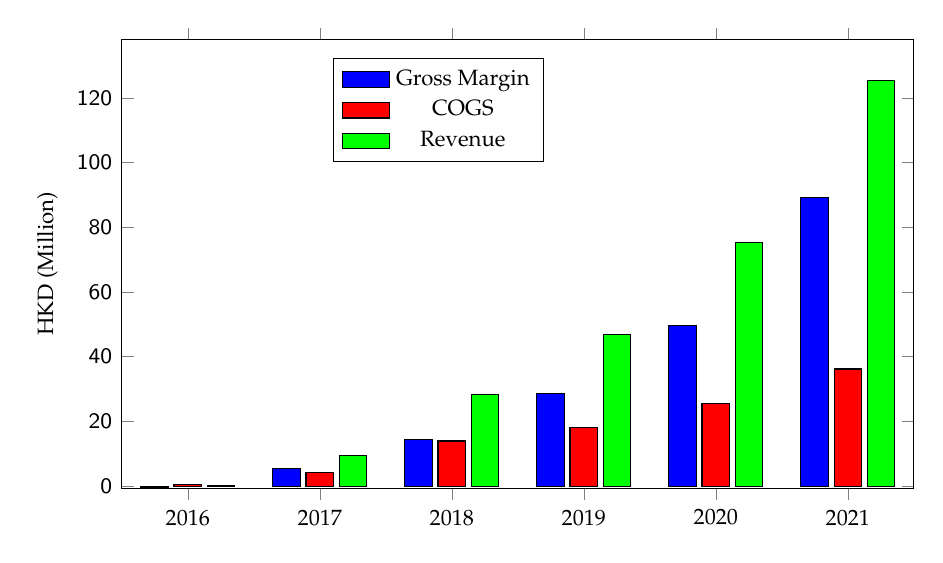
\begin{tikzpicture}
\begin{axis}[
width=0.96\linewidth,
height=0.60\linewidth,
%ybar stacked,
ybar,
area legend,
legend style={at={(0.4,0.96)}, anchor=north},
symbolic x coords={2016, 2017, 2018, 2019, 2020, 2021},
xtick=data,
ymin=-0.6,
ylabel=HKD (Million),
enlarge x limits=0.1
]
\addplot[ybar,fill=blue] coordinates {
    (2016, -0.400000) (2017, 5.36) (2018, 14.443) (2019, 28.688) (2020, 49.758) (2021, 89.177)
};
\addplot[ybar,fill=red] coordinates {
    (2016, 0.500000) (2017, 4.24) (2018, 13.957) (2019, 18.072) (2020, 25.506) (2021, 36.193)
};
\addplot[ybar,fill=green] coordinates {
    (2016, 0.100000) (2017, 9.6) (2018, 28.4) (2019, 46.760) (2020, 75.264) (2021, 125.3696)
};
\legend{Gross Margin, COGS, Revenue};
\end{axis}
\end{tikzpicture}
	\caption{Rough financial projections of Pear in 5 years.} \label{fig:financial-projections}
\end{figure}

\subsubsection{Exit Strategy and IRR}
Table~\ref{tb:exit-strategy-irr} shows the exit strategy and the corresponding return rate. 
\begin{table}[htbp]
	\centering
	\caption{Exit Strategy and IRR}\label{tb:exit-strategy-irr}
	\begin{tabular}[t]{lrrr}  
		\toprule
		Cases & Optimistic & Baseline & Pessimistic\\
		\midrule
		Exit Strategy & IPO & Buy Back & M\&A\\
		NPV (HKD) & 355,829,000 & 33,778,000 & 5,648,000\\
		IRR & $242\%$ & $93\%$ & $51\%$\\
		\bottomrule
	\end{tabular}
\end{table}

\subsubsection{Use of Investment}
Table~\ref{tb:use-of-investment} shows the use of investment which can be roughly divided into four parts.  
\begin{table}[htbp]
	\centering
	\caption{Use of Investment}\label{tb:use-of-investment}
	\begin{tabular}[t]{ccccc}  
		\toprule
		Total & Pilot \& Field testing & R \& D & Marketing & G \& A\\
		\midrule
		$6,000$ K & $1,500$ K & $3,800$ K & $500$ K & $200$ K\\
		\bottomrule
	\end{tabular}
\end{table}

In this recession \& capital winter, Pear will spend about two-thirds of its Series Pre-A round funding on R\&D, in order to build finely crafted products, competitive advantages and barriers to market entry. 
This long-term investment will generate unexpected results in ``winter to spring'', when there will be a lot of cheap resources ({\em e.g.} dying O2O companies' legacies) available to obtain.

\newpage

\chapter{Historical Analysis}\label{chp-his-analysis}
If you want to predict the future, go look into the past\footnote{In business schools, we usually only learn about things that have happened in the past; here we also analyse what is happening now and what will possibly happen in the near future.}. 

In this chapter, we first seek to go back in time machine to take a retrospective view of the history concerning related fields, from a combination of industrial and academic perspectives. Then, we do some analysis, analysing technologies that emerged, why they became standards and why some were unsuccessful in the end. We also state practical lessons we have learned from this history and how these have inspired our decisions, resolutions and solutions\footnote{We only talk about the technologies that are general-purpose, and have made a difference or will potentially change the world in multiple areas to a great extent. We discuss domain-specific technologies, techniques, applications and phenomena in the respective following chapters.}.
%define the core problems which inspires and unveils  
% push our thinking to get the root causes

\section{Network Protocol and Efficiency}\label{sec-his-analysis-tcp}
The ancestor of today's Internet was the ARPANET, a military project established by DARPA (the then ``ARPA'') of the US Department of Defense (DOD) in 1969. Its primary goal was to decentralise the command and control processing and switching so the communication network could survive a nuclear attack. In the beginning, ARPANET used a simplex protocol called the Network Control Program (NCP) for communication between host computers. 

In 1983, the Transmission Control Protocol / Internet Protocol (TCP/IP) suite replaced NCP as ARPANET's principal protocol, and ARPANET then became a part of the early Internet. According to statistics from different parties, TCP accounts for 60\% to 95\% of the wide-area Internet traffic. 

TCP uses a decent ``gentleman'' congestion control mechanism \cite{Chiu:1989:AIMD} that guarantees long-term fairness among competing connections. It does not rely on the routers (intermediate nodes) to give any feedback information about network conditions to the source. This end-to-end elegency\footnote{Similar scenarios also exist in Artificial Intelligence and Deep Learning: if an end-to-end solution is developed, it is more likely to be shortly accepted and widely deployed to solve general or domain-specific real-world problems.} reminds of another story. 

Ethernet/TCP/IP is adequate in many data transmission scenarios, but inadequate for Quality of Service (QoS) guaranteed telecommunication applications. Thus, intermediate network nodes were considered to be used to provide feedback regarding congestion status. In the 1990s the Asynchronous Transfer Mode (ATM) was popular as a protocol stack that worked on multiple layers that actualised such mechanism. At that time, ATM attracted much investment and research interest. However, it almost died and was replaced by Ethernet/IP in most public networks at the beginning of this millennium. Below we try to list some reasons: 
% makes us recall another story (which required every node adds feedback field to imply the end the congestion status) in the evolution of the Internet protocol stack.

\begin{description}
	\item[High Complexity and High Cost] Compared with Ethernet/IP, ATM was more expensive in terms of the required hardware and manpower for operation. It also required more time to train people to become experts. 
	\item[Weak Value Proposition] The development of statistical multiplexing technologies overshadowed the advantages of ATM. Although Ethernet/IP networks originally could not guarantee a high degree of QoS, this factor diminished over time as statistical multiplexing technologies improved.  
	\item[Weak Interoperability] Ethernet created a sustainable eco-system: it supported an open, multi-vendor and cross-platform environment; ATM did not. An existing ATM switch would probably not interoperate with one from a second vendor. This meant that after purchasing an ATM switch from one vendor, the user was locked into that supplier. 
	\item[Weak Upgradeability] It is easy to upgrade Ethernet to 100 Mbit/s, to 1Gbit/s, and even 10Gbit/s, while upgrading ATM requires all legacy software to be changed. Eventually, Ethernet won the speed race in LAN over ATM: 100BaseT Ethernet kicked out 25 Mb/s ATM in the desktop; 1Gbps/10Gbps Ethernet wiped out ATM on the campus. 
	\item[Weak Profitability to Most Parties] Only the telephone companies were active in deploying ATM networks. The reason was quite simple: to count the bits a customer generated/consumed in the established end-to-end connection conveniently and charge him accordingly.  
	\item[Slow in Touching Ground in the Market and Industrial Standardisation] Network operators would be required to change the infrastructure, since in the LAN world IP and Ethernet first took hold as the \textit{de facto} standards, and equipments based on these standards were so much simpler, easier to understand and significantly cheaper than the corresponding ATM equipments.
\end{description}

It is known to all networking professionals that Equation~\ref{throughput:formula:tcp}  below is the throughput TCP can achieve at a steady state; Equation~\ref{throughput:formula:tcp:max} is roughly the maximum throughput TCP can achieve. 
\begin{equation}\label{throughput:formula:tcp}
Throughput_{TCP} = \frac{\min\{RWND, CWND\}}{RTT}
\end{equation}
\begin{equation}\label{throughput:formula:tcp:max}
Throughput_{TCP_{max}} = \frac{RWND_{max}}{RTT}
\end{equation}
where $RWND$ is the receiver window size, $CWND$ is the congestion windows size (at the sender side), and $RTT$ is the round trip time. 

Also, theoretically we have Equation~\ref{throughput:formula:tcp2} if considering the loss rate $p$. 
\begin{equation}\label{throughput:formula:tcp2}
Throughput_{TCP} \sim \frac{1}{RTT} \sqrt{\frac{3}{2p}}
\end{equation}

Let's consider transmitting a data chunk from node $A$ to node $B$. When the distance between $A$ and $B$ gets longer, generally the $RTT$ is larger for a certain type of transmission medium. In addition, $p$ is also likely to be larger, as there are likely to be more routers along the path from $A$ to $B$, and their performance, buffer window sizes, and current congestion status may vary. Thus, any single node in between can be a bottleneck. 

In addition to the window sizes, the packet loss rate $p$, and the $RTT$, there are other factors that affect TCP's performance: the slow-start and the 3-way handshake behaviour. 

The 3-way handshake introduces one more factor in RTT latency. To eliminate this, Google proposed TCP Fast Open (TFO) \cite{rfc7413}. When a client reconnects to a server it has connected to before, it sends an initial SYN packet along with a TFO cookie (which was generated by the server using a block cypher over the client's IP address) to authenticate itself. If this is successful, the server may start sending data to the client even before the reception of the final ACK packet of the three-way handshake. Linux Kernel implemented a full support of TFO in version 3.16\footnote{\url{http://kernelnewbies.org/Linux_3.16}}, and Microsoft's Edge browser has supported it since late May of 2016\footnote{\url{https://developer.microsoft.com/en-us/microsoft-edge/platform/changelog/desktop/14352/}}, although the adoption process still seems slow. 

Due to severer eavesdropping, tampering and pretending by 3rd-parties in the middle of a connection, more and more web service providers (oftentimes using HTTP) have started to enable a Transport Layer Security (TLS) layer on top of TCP. However, a typical (TCP + TLS) model would cause two to three RTTs' latency before actual data transmission. To eliminate these, Google proposed QUIC \cite{tsvwg-quic-protocol-02}, which is built on top of the User Data Protocol (UDP). It is currently supported by Google Chrome by default when connecting to Google's servers. Nevertheless, Google's current implementation of QUIC is still in a transitional form, as TLS 1.3 is not ready; it uses some tricks to fulfil the ``0-RTT'' handshake. 
% another paragraph?

The 1 or 2 Maximum Segment Size (MSS) of the initial $CWND$ makes TCP very slow in its slow-start phase. Google proposed changing this value to 10 in \cite{rfc6928}. As it is simply a one-value tuning, it is now adopted by almost all Linux- and OpenBSD-based operating systems. 

Over one decade ago, there were a bunch of start-up companies trying to improve TCP throughput by adding a tricking field in the header storing feedback information from specially designed routers. Unfortunately, none of these companies survived. 

Recently, there has been a China-US company called AppEx\footnote{\url{http://www.appexnetworks.com/}} doing the same thing but at a single end (usually deployed on the server side). They use a learning-based \cite{zhuang2014optimization} approach to adjust $CWND$, resulting in near-optimal, smooth and stable throughput over time. ServerSpeeder, AppEx's core product which contains a Linux kernel patch, has been adopted by a considerable number of business users including Huawei and ChinaCache. These deployments potentially prove it a successful business. 

In additional to the improper setting of buffer sizes, there is another cause why TCP is unable to ``fill up the pipe'' in long-haul backbone connections: high transmission error rate. Since TCP lacks an error-nature classification mechanism, the congestion window can be halved unnecessarily when there is a packet loss caused by bit errors. To address these problems in inter-continental VPNs, Homing Systems \footnote{\url{http://www.homingsystems.com/}} developed a reliable proxy and gateway based on UDT \cite{Gu:2007:UDT}, which was a reliable transmission protocol built above UDP. In their real-world testing results, a 5-10x speedup can often be reached when transmitting data between China and the US. 

From the rise and fall of the above protocols, we learned five valuable lessons: 
\begin{enumerate}
	\item Do not rely on the changes at both ends; 
	\item If there is an inevitable change, work on a single and easier-to-deploy end; 
	\item Do not attempt to change the existing fundamental infrastructure that is already widely deployed;
	\item Instead, try to build upper-layer protocols on top of the fundamental ones;
	\item Otherwise, do something helpful but orthogonal.
\end{enumerate}

\section{HTTP, HTML, and the Web}\label{sec-analysis-http}

When a considerable number of computers were connected, people became willing to compose and share content. To make the generating, publishing, and consuming of content easier, Tim Berners-Lee started the now well-known project called the World Wide Web (WWW, 3W, W3, or the Web) in 1989. In that project, HTTP for data request-response, HTML for data representation, as well as URL for resource locationing were defined. The first well-accepted version, HTTP 0.9, was documented in 1991. HTTP 1.0 \cite{rfc1945} was finalised in May 1996 but was then replaced by HTTP 1.1 \cite{rfc2068} in 1999. 

Around that time, as more and more sites were set up and more and more content was generated, the searching and retrieval of information in HTML Web Pages became a big issue. Google won the battle among all the competition, because it worked in cooperation with the CIA \cite{google-cia} and was able to develop reliable distributed systems like GFS and algorithms like PageRank that made almost the whole process fully automated. The early stage of Google could be seen as an automated miner and ranker over the content composed by HTML and delivered via HTTP. 
% Before that time, there was another popular protocol Gopher...  -- address the power of standards
% need info. about HTTP2 ???
% Facebook built on Web2.0  PHP, MySQL...
Another CIA front company that has become an Internet giant, Facebook \cite{fb-cia}, built its social network service on top of HTML 4.01, an easier ``composer'' and gateway --- PHP, and an open source DBMS --- MySQL. 
In 2008, after the WHATWG of W3C published the first working draft of HTML5, Facebook was the first giant to fully embrace HTML5. However, a few years later, Mark Zuckerberg admitted that the biggest mistake Facebook had made was betting too much on HTML5\footnote{\url{http://techcrunch.com/2012/09/11/mark-zuckerberg-our-biggest-mistake-with-mobile-was-betting-too-much-on-html5/}} rather than native applications. Although HTML5 is now very popular for developing mobile-friendly websites and even applications, in 2008 the supporting technology simply was not ready. This was due to two major factors: 

\begin{enumerate}
	\item HTML5 is an enormous standard that contains too many details related to too many fields.\\
	In 2008, building a cross-platform HTML5 engine from scratch was not a trivial work. Besides, the quality and performance could not be easily guaranteed. 
	\item The then mainstream hardware was still too weak to support smooth user interaction for HTML5.\\
	Compared with using native programs, the user experience was just intolerable. 
\end{enumerate} 

However, after four or five years, HTML5 development was a good idea thanks to advances in mobile computing devices and browser engine implementations.

% Simply, if Facebook did the shift to pure HTML5 development fashion 4 or 5 years later, the results would be totally different.
From this historical analysis, we learned three valuable lessons: 
\begin{enumerate}
	\item The timing for embracing a new technology is important; 
	\item Front organisations for intelligence gathering agencies tend to be trendsetters;
	\item These organisations can get away with timing mistakes, but others often cannot. 
\end{enumerate}  

\section{P2P, CDN, Cloud}
Before Berners-Lee invented the Web, the Internet was a bit more than if not merely a set of linked computers. But after that, the Internet enjoyed explosive growth in both content volume and traffic demand. Around 1995, Internet services very often suffered from the ``hot-spot'' (aka ``flash-crowd'') and the ``bottle-neck'' problems, which became potential barriers that could seriously stop the growth of the Web. Berners-Lee then organised a challenge at MIT to improve the method of Internet content delivery. Among those who were involved in the challenge, there was a graduate student named Daniel Lewin, who devised a key method called \emph{Consistent Hashing} \cite{Karger:1997:Consistent} and started a company called Akamai, which became the world's largest Content Delivery Network (CDN) service provider. On 11 September 2001, Lewin scheduled a visit to a young guy named Travis Kalanick for a potential investment deal. Kalanick\footnote{8 year later, he founded Uber --- the largest sharing economy company and the most valuable start-up.} was solving similar problems using a different technology called P2P. Unfortunately, Lewin's flight was hijacked, and he became the first victim in the 9/11 Attacks. 

The basic idea of a CDN is to deploy servers in multiple geographically diverse locations over data centres of multiple ISPs ({\em i.e.} $<ISP, region>$ touples) across the Internet. The system redirects users' requests to enable short (network topological) distance transmission. 

Around 2005, P2P network applications became popular and lasted for a while. In P2P, the nodes are not categorised as Client/Server (C/S). Instead, every peer can receive data from and serve data to others simultaneously. From an applications perspective, P2P was used for file downloading first, then Voice over IP (VoIP) and live streaming, succeeded by Video on Demand (VoD), and video conferencing as well. P2P could largely solve the bandwidth bottle-neck problems on Content Providers' (CPs') servers and ISPs' backbone networks. As the longer time a P2P program stays online, the more traffic it helps the servers save, many P2P software applications worked as background programs (aka daemons) and start-up processes. In the commercialisation process that followed, this always-stably-online feature became attractive to many P2P companies, which just leveraged this feature to do advertising. Unfortunately, some added malicious or obnoxious advertising or marketing or spying functionalities to their existing software. Annoyed by this, end-users became unwilling to install any stand-alone application to their PCs. In China, the rise of Qihoo 360 Security Guard and QQ PCMgr accelerated the speed of this software being blacklisted. 

Apart from the bad reputation due to malware, almost all then popular P2P software faced a serious legal problem --- copyright infringement. Below is an incomplete list of famous P2P practices:  
% Rises and Falls of P2P practices
\begin{description}
	\item[KaZaA] Lost all the copyright lawsuits in Australia and the US from 2004 to 2006. Not long after a settlement of USD 100 million in reparations to the recording industry, KaZaA ended its service. Identified as a spyware application by StopBadware.org in 2006.  
	\item[Popcorn Time] Forced by Hollywood to close on 21 October 2005. Even its source code was deleted later on. 
	\item[BTChina] Closed all services on 6 December 2009, forced by the State Administration of Press, Publication, Radio, Film and Television of China. 
	\item[VeryCD] Deleted all eD2k links in its music and movie sections. Closed its movie downloading functionalities on 30 June 2011. Deleted all eD2k links in September 2012. 
	\item[QVoD] Chinese Police raided its headquarters on 22 April 2014. All servers were seized. Xin Wang, the CEO of QVoD, was arrested on 8 August 2014 in South Korea. The main reason was its pornographic and pirated content. 
	\item[The Pirate Bay] In response to a complaint from a Swedish anti-piracy group, police in Stockholm raided the company's premises and seized servers and other equipment on 9 December 2014. 
\end{description}

Why the above P2P applications all failed or disappeared eventually? Were they doing self-pleasure? Figure~\ref{fig:p2p-fail-root} is a root-cause-like analysis of the failures of P2P practices. 
\begin{figure}[ht]
	\centering
	\includegraphics[width=1.00\textwidth]{fig/his-analysis/p2p_fail_analysis.pdf}
	\caption{Root-Cause-like Analysis of P2P Failures}\label{fig:p2p-fail-root}
\end{figure}

By the way, in industry there were a few quite successful ones, like BitTorrent and Gnutella. There might be two factors. First, they did not emphasise too much on the search functionality, which on the other hand prevented the developers and operators from legal threads. Second, they had rather cooperate with CPs and serve as a middleware to help them reduce content distribution cost. 

Around 2009--2010, CDN companies started to apply multi-layered architectures and purchase storage and computing resources from data centres and edge servers at wholesale and sell them to service users (Internet Content Providers, such as Yahoo, Youtube and Facebook) at retail. CDN seemed like a potential winner in this networking battle. 

Distributed storage is an important sub-system of CDN, but this technology catalysed a bigger thing which became a super-set of CDN --- the Cloud. Distributed Hash Table (DHT) was originally designed for P2P systems, but some modifications of it like \cite{DeCandia:2007:Dynamo} later served as a core component in most clouds. 

When the Cloud first appeared, many researchers thought that it was merely ``old wine in a new bottle'': it is essentially identical to Grid Computing. Less than one decade later, the Cloud has now almost taken over the world. Two intrinsic attributes of the Cloud are its business friendliness and its \emph{as-a-service} thinking, while Grid Computing was only ``played'' by researchers for scientific projects. 
%Apart from the methods described in Section xxx, there are a few other approaches also able to . 
%http://www.businessinsider.com/uber-travis-kalanick-bio-2014-1

In 2001, Bill Joy, Sun's co-founder and chief scientist, announced the JXTA\footnote{\url{https://jxta.kenai.com/Specifications/Specifications.html}} project at the O'Reilly Peer-to-Peer Conference. ``Project JXTA fulfils a vision I've had for 25 years,'' said Joy. 
JXTA used a 128-bit UUID to identify all the entities ({\em e.g.} peers, advertisements, services) in the network. A peer is a virtual communication point, and one physical node can have multiple peers. Endpoint is another abstraction that describes the address that helps fulfil a peer-to-peer communication in a certain protocol. An advertisement is an XML document ``name card'' that describes a peer, a peer group, a pipe, a service, or any resource. A Rendezvous Peer cooperates with other Rendezvous Peers and with client peers to propagate messages amongst the peers of a peer group, which helps with the publishing and retrieval of advertisements. The most creative feature of JXTA is its pipe, which can help peer-to-peer communication even if a direct connection cannot be built due to firewalls and NATs in between. 

JXTA defined a suite of six protocols base on XML: 
\begin{description}
	\item[PRP] Peer Resolver Protocol. A core protocol that provides a generic query/response interface. It is a fundamental protocol that supports PDP, PBP, and PIP. 
	\item[ERP] Endpoint Routing Protocol. The other core protocol that helps a peer route messages to their destination. It helps traverse the firewalls and NATs if they exist along the path. 
	\item[PDP] Peer Discovery Protocol. To discover any published resource (represented as an advertisement).  
	\item[RVP] Rendezvous Protocol. For propagation of messages within a peer group.  
	\item[PIP] Peer Information Protocol. For obtaining the status information of other peers, including uptime, inbound and outbound message count, and the time the last message is sent and received. 
	\item[PBP] Pipe Binding Protocol. Layered upon the ERP, PBP helps peers to build virtual communication tunnels (pipes).  
\end{description}

JXTA was an ambitious project that aimed at building a unified P2P platform (or middleware, to be more precise) to make P2P application development easier. 

However, in the following years, JXTA was ignored by enterprises, believing it was a pure ``Joy's project''.  Only struggling community volunteers were maintaining JXTA projects. A few applications developed by volunteers did exist, but none of them eventually amounted to anything. 

Sun had progressively reduced its contributions to JXTA since 2008, before its acquisition by Oracle. In November 2010, Oracle officially announced its withdrawal from JXTA projects. What was worse, JXTA even failed in being moved to the Apache Software Foundation, as Oracle did not reply anything on the licence issue and the members on board did not organise elections by the open-source community. No one cared about its future and destiny. 

Below are lessons we learned from JXTA: 
\begin{itemize}
	\item Too many objectives.\\
	It tried to construct a unified platform that includes everything but in fact, it addressed none of them. 
	\item Still lacked compelling-needed application-layer features.\\
	Before 2008, it could not automatically handle peer group management; it did not address the scalability problem: it did not support hierarchical peer-groups; it did not handle dynamic peer groups well; it had no security guarantee; it had no convenient directory functionalities; it did not even support UDP. 
	\item Could not find its place in either technology or business.\\
	It looked more like a service oriented framework, but it was indeed a middleware. It did not create an ``XaaS'' platform, let alone a business-friendly ecosystem. 
	\item Too complex for the developers.\\
	As a P2P development library, it was too difficult to use. The exposed APIs were not well designed and organised, and coupling with its internal logic processes. 
	\item Wrong technology choices.\\
	It is true that XML is an international standard. But using XML in all layers is insane. This would also create much overhead. In addition, JXTA was friendly to the J2EE community but not to the networking community. That latter was truly the main force in developing P2P applications.   
	\item Low performance in serving any specific scenario.\\
	\textsl{VOIP} looks for relay performance and reliability, while \textsl{VoD} emphasises average throughput. Furthermore, \textsl{Live Streaming} needs low delay and \textsl{File Sharing} stresses resource coverage. JXTA addressed none of them. Above all, it had a very long start-up time. 
	\item No industrial standardisation work.\\
	The JXTA community had never filed any standard proposals to any influential standardisation organisation or institution, let alone attracted any standardisation group being assigned working on it. 
\end{itemize}
 

\section{C10K and C10M Problems}
In 1999, handling ten thousand clients concurrently  was a challenge for a web server. People coined it --- ``the C10K problem''\footnote{\url{http://www.kegel.com/c10k.html}}. A straightforward solution was to process the connections using multiple tasks (processes or threads). However, due to the overhead of task scheduling and management, this method was not scalable. Then people turned to models that handle multiple connections in one process/thread. In the following years, nonblocking, multiplexing, signal driven and asynchronous I/O models were proposed and implemented in modern operating systems. 

Since 2010, the web server Nginx, which supports multiple I/O models, has been widely deployed, so the C10K problem seems to be resolved\footnote{There are several other milestones, but we believe the Nginx one is the most significant.}. 
% the wisdom in epool and kqueue is the use of callback functions  

But good times do not last long. As the number of connected devices increases and the applications becomes more and more complicated, we will soon face a new problem, C10M\footnote{\url{http://c10m.robertgraham.com/p/manifesto.html}}. That is, handling 10 million concurrent connections to one server. This new problem seems more challenging. Proposed solutions have included co-routine, asynchronous callback, per-CPU data structures, lock-free algorithms, memory scaling, and Non Uniform Memory Access Architecture (NUMA). MigratoryData has even announced that they have successfully scaled to 12 million connections\footnote{\url{https://mrotaru.wordpress.com/2013/10/10/scaling-to-12-million-concurrent-connections-how-migratorydata-did-it/}}. 

The above progress have given us a useful indication: designing a fully distributed model might be not necessary for some scenarios in the future. 

\section{Distributed Generation versus Distributed Computing}\label{sec-dg-vs-dc}

During the past century, many power companies have attempted to do distributed generation. But up until today, we still have not seen it widely deployed. ``Distributed generation wasn't successful in 1900. It wasn't successful in 1950. It wasn't successful in 2000. And it won't be successful in 2050,'' said Joe Welch, the founder and CEO of ITC Holdings, the largest transmission-only company in the US\footnote{\url{http://www.utilitydive.com/news/itc-holdings-ceo-distributed-generation-will-never-beat-centralized-grid/}}. As a distributed fog shares a lot of properties with the distributed generation paradigm, some people may question if Fog Computing will be successful from a similar perspective. In this section, we analyse the differences between distributed generation and distributed computing. 

\begin{enumerate}
	\item Distributed generation is less efficient than its centralised counterpart, but the Fog is more efficient than the Cloud concerning performance per unit of cost.\\
	In power generation, the bigger the generator system is, the more the energy transformation ratio is. 
	This is why power companies have not only been continuously increasing the capacity, the diameter and the speed of motors but have also been keen on building engineering miracles like the Three Gorges Dam and the Itaipu Dam. 
	However, in computing, the bigger the processor is, the lower power efficiency the system has. In recent years, the per-chip performance of desktop and server CPUs have not improved much\footnote{Compared to Moore's Law, which states that performance doubles every 18 months.}, but their power efficiency has taken great leaps forward. 
	
	Over the last few years, minimising non-computing or ``overhead'' energy has become the biggest issue in data centre research. Only a few years ago, data centres used almost as much non-computing energy (for example, for cooling, air movement, and power conversion) as they did to power their servers \cite{Weihl:2011:SDC}. On the contrary, in the Fog, as the nodes are usually deployed in spacious places, we do not need to set up additional pieces of equipment to cool them off. 
	
	Figure~\ref{fig:spec-performance-power} shows some results of a SPEC2006 benchmark test over several different CPU series done in early 2016\footnote{For comparison convenience, all platforms were adjusted to 16nm 1MB L2\$/LL\$ per core and 16nm per industry scaling metrics. Data source: \cite{soft-visc}.}. It is clear that for all series, as the performance increases, the power grows exponentially. 
	%\begin{figure}[ht] 
	%		\centering 
	%		\subfigure { \label{fig:cpu-efficiency} 
	%			\includegraphics[width=0.48\linewidth]{fig/his-analysis/visc_engergy.png} 
	%		} 
	%		\subfigure { \label{fig:spec-cpu-performance} 
	%			\includegraphics[width=0.48\linewidth]{fig/his-analysis/visc_single_thread.png} 
	%		}
	%		\caption{A SPEC CPU 2006 Test in Early 2016.} 
	%		\label{fig:spec-performance-power} 
	%\end{figure}
	\begin{figure}[ht] 
		\centering 
		\input{fig/his-analysis/arm_apple_intel}
		\caption{SPEC2006 Single Thread Score versus Watt (16nm).} 
		\label{fig:spec-performance-power} 
	\end{figure}
	
	Such phenomena not only exist in CPUs, such as ARM Cortex\footnote{\url{http://forums.anandtech.com/showthread.php?t=2208184}}, but also in GPUs such as nVIDIA GTX \cite{gtx-1080}. Figure~\ref{fig:performance-power-cpus-gpus} plots some of the benchmark results.
	%\begin{figure}[ht] 
	%		\centering 
	%		\subfigure[Performance vs. power of ARM CPUs.] { \label{fig:arm-pp-cortex} 
	%			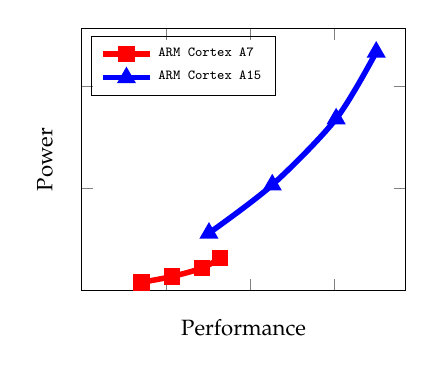
\begin{tikzpicture} %[>=latex]
\begin{axis}[
width=0.47\textwidth,
%line width=2,
%symbolic x coords={2012, 2013, 2014, 2015, 2016},
xticklabels={,,},
yticklabels={,,}
%xticklabels={720p,1080p,4k},
%minor xtick={0,1,...,18},
grid=both,
ymin=0,
xmin=0,
xlabel=Performance,
ylabel=Power,
legend pos=north west,
legend cell align=left,
legend style={
	font=\tiny,
	fill=none,
	%/tikz/column 2/.style={
	%	column sep=5pt,
	%},
},
%enlarge x limits=0.1,
%xticklabel style={text width=0.2\textwidth,align=flush left},
]
\addplot[line width=2pt,smooth,color=red,mark=square*] coordinates {
	(20/28,3/18)
	(30/28,5/18)
	(40/28,8/18)
	(46/28,11.5/18)
};
\addplot[line width=2pt,smooth,color=blue,mark=triangle*] coordinates {
	(42.3/28,20.3/18)
	(63.3/28,37.3/18)
	(84.5/28,60.6/18)
	(97.8/28,84.1/18)
};
\legend{\texttt{ARM Cortex A7~}\\\texttt{ARM Cortex A15}\\}
%\draw[red] plot [smooth] coordinates {(0 0) (2,3700) (4,6006) (18,18000)};
\end{axis}
\end{tikzpicture}
	%			%\includegraphics[width=0.46\linewidth]{fig/his-analysis/arm_cortex_a7_a15.jpg} 
	%		} 
	%		%\subfigure[Performance vs. power of nVIDIA CPUs.] { \label{fig:nvidia-pp-gtx} 
	%		%	\includegraphics[width=0.50\linewidth]{fig/his-analysis/gtx_gpu.jpg} 
	%		%}
	%		\subfigure[Performance vs. power of nVIDIA CPUs.] { \label{fig:nvidia-pp-gtx} 
	%			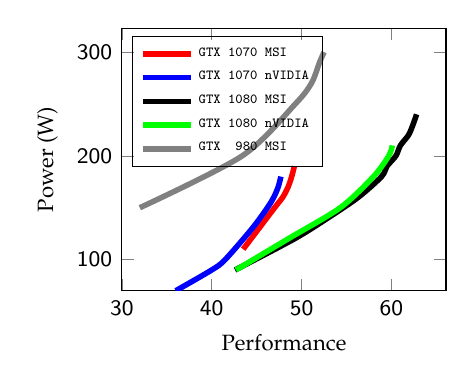
\begin{tikzpicture} %[>=latex]
\begin{axis}[
width=0.47\textwidth,
%line width=2,
%symbolic x coords={2012, 2013, 2014, 2015, 2016},
%xticklabels={,,},
%yticklabels={,,}
%xticklabels={720p,1080p,4k},
%minor xtick={0,1,...,18},
grid=none,
xmin=30,
ymin=70,
xlabel=Performance,
ylabel=Power (W),
legend pos=north west,
legend cell align=left,
%legend columns=2, 
legend style={
	font=\tiny,
	fill=none,
	%/tikz/column 2/.style={
	%	column sep=5pt,
	%},
},
%enlarge x limits=0.1,
%xticklabel style={text width=0.2\textwidth,align=flush left},
]
\addplot[line width=2pt,smooth,color=red] coordinates {
	(43.5,110) (47,150) (47.9,160) (48.5,170) (48.9,180) (49.2,190)
};
\addplot[line width=2pt,smooth,color=blue] coordinates {
	(36,70) (40,90) (41.5,100) (44.5,130)
	(46.2,150) (46.9,160) (47.4,170) (47.7,180)
};
\addplot[line width=2pt,smooth,color=black] coordinates {
	(42.6,90) (49.2,120) (52.9,140) (56.3,160) (58.9,180) (59.5,190)
	(60.5,200) (61.0,210) (61.9,220) (62.4,230) (62.8,240)
};
\addplot[line width=2pt,smooth,color=green] coordinates {
	(42.7,90) (48.5,120) (54.3,150) (58.0,180) (59.7,200) (60.1,210)
};
\addplot[line width=2pt,smooth,color=gray] coordinates {
	(32.0,150) (43.4,200) (49.3,250) (51.1,270) (52.0,290) (52.5,300)
};
\legend{\texttt{GTX 1070 MSI}\\\texttt{GTX 1070 nVIDIA}\\\texttt{GTX 1080 MSI}\\\texttt{GTX 1080 nVIDIA}\\\texttt{GTX ~980 MSI}\\}
%\draw[red] plot [smooth] coordinates {(0 0) (2,3700) (4,6006) (18,18000)};
\end{axis}
\end{tikzpicture}
	%		}
	%		\caption{Performance vs. power of CPUs and GPUs.} 
	%		\label{fig:performance-power-cpus-gpus} 
	%\end{figure}
	\begin{figure}[ht]
		\begin{minipage}[t]{.50\linewidth}
			\centering
			\input{fig/his-analysis/arm-cortex-cpu2}
			\centerline{\parbox[t]{\linewidth}{\centering\footnotesize (a) Performance vs. power of ARM CPUs.}}
		\end{minipage}
		\hfill
		\begin{minipage}[t]{.50\linewidth}
			\centering
			\input{fig/his-analysis/gtx-gpu2}
			\centerline{\parbox[t]{\linewidth}{\centering\footnotesize (b) Performance vs. power of nVIDIA CPUs.}}
		\end{minipage}
		\caption{Performance vs. power of CPUs and GPUs.}
		\label{fig:performance-power-cpus-gpus} 
	\end{figure}
	
	Blem {\em et al.}~\cite{Blem:2015:ISA} did comprehensive benchmark tests over multiple commodity ARM, x86, and MIPS CPUs. Figure~\ref{fig:power-performance-isa} shows some of their results. 
	\begin{figure}[ht] 
		\centering 
		\subfigure[Tech-independent average power normalized to A8.] { \label{fig:tech-independent-avg-power} 
			\includegraphics[width=0.44\linewidth]{fig/his-analysis/avg-power_to_a8.png} 
		} 
		\subfigure[Power performance tradeoffs.] { \label{fig:power-performance-tradeoffs} 
			\includegraphics[width=0.52\columnwidth]{fig/his-analysis/power-performance_tradeoffs.png} 
		}
		\caption{Power and performance of different CPU architectures.} 
		\label{fig:power-performance-isa} 
	\end{figure}
	
	If we replace the lateral axis to cost in monetary units, the curve will remain a similar shape. 
	
	Usually, cloud uses high-performance chips while fog uses low-power ones. If we can achieve near-linearly scaling, fog surely will be more cost and energy efficient. 
	
	\item The problems of distributed power generation are ``hard'', while ``soft'' in fog.\\
	To integrate with the grid and interoperate with other systems, there are problems like synchronisation and voltage control remaining to be solved. All of them require replacement of hardware. In contrast, most fog problems lie in the software layer and can be easily solved by complying with unified protocols. 	
	\item Interoperability.\\
	Due to rate, frequency, voltage, availability, reliability and operational management issues, integrating distributed generation to the electricity grids has always been a non-easily solvable issue.  
	\item The desirability of distributed generation is much weaker than that of fog computing.\\
	Recent technologies like UHV (Ultra-High-Voltage) electricity transmission have heavily reduced the desirability of distributed generation. However, because of the RTT-throughput relationship and fog's inherent proximity to the sensors at a local environment, the demand for fog computing keeps growing. 
	
\end{enumerate}

Therefore, it is clear that expectations regarding the future of distributed computing should not be based on the history of distributed generation.  
% http://www.greentechmedia.com/articles/read/the-energy-blockchain-could-bitcoin-be-a-catalyst-for-the-distributed-grid
%http://www.forbes.com/sites/williampentland/2016/06/27/bracing-for-blockchain-distributed-ledgers-poised-to-drive-adoption-of-distributed-generation/

\section{CCN and ICN}\label{sec:icn}
Historically, compared with servers and PCs, routers have usually had smaller memory. This has been due to cost considerations as well as properties of the Internet:
\begin{enumerate}
	\item The ``store-and-forward'' nature of the Internet infrastructure.\\
	The Internet was designed and built on top of existing telecommunication systems. In telecommunications, the ``store-and-forward'' principle and technique had been applied almost everywhere. 
	\item The packet loss rate does not improve much as the buffer size keeps increasing.\\
	The packet loss rate (which is simply equal to buffer overflow probability in most cases) is a negative exponential function of the buffer size. 
	From Anick's \cite{Anick1982Stochastic} and Guerin's \cite{Guerin1991Equivalent} works, it is not hard to derive Equation~\ref{eq:packet-loss-rate}, which satisfies both the finite and the infinite buffer assumption models, just with different values of $A$. 
	\begin{equation}\label{eq:packet-loss-rate}
	\epsilon \approx A\mathrm{e}^{-Bx}
	\end{equation}
	where $\epsilon$ is the loss rate and $x$ is the buffer size. 
	
	Therefore, according to these theories, the buffer memory requirement of routers does not increase much with upgrades in QoS level or link capacity. 
\end{enumerate}
	As the primary usage of the Internet has transformed from host-centric, end-to-end communication (to find the address of a host in order to fetch certain data) to content retrieval (no matter where the data is), the traditional TCP/IP model has become more and more inefficient. Attempts to improve the model without changing the substrates have merely complicated things, as they have introduced ``patching-over-patching'' requirements. The advent of CDN was just one such example. Thus, in recently years, researchers have proposed Information-Centric Networking (ICN) \cite{Xylomenos2014ICN} architectures, such as Content-Centric Networking (CCN) \cite{Perino:2011:CCN}. In these architectures, information is the focal point, and it is named and decoupled with location. All routers (intermediate nodes) along the transmission paths deterministically cache, manage, and replace the transmitted data, thus improving the content retrieval efficiency and network resource utilisation in a transparent, ubiquitous, and fine-grained way for the receivers. 
	
	It is believed by many researchers that these models might revolutionise the Internet infrastructure in 15 years, although with significantly challenging difficulty and the prerequisite of replacing all current routers. 
	
	The understanding is that routers in these architectures shall be equipped with large memory size and large storage capacity in order to handle increased responsibilities. 
	
	Before the potential adoption of ICN, the advent of smart routers (see Section~\ref{sec-smart-routers}) suggests that in the future even most edge routers would be powered with large buffering or storage capacities. 
	
    Furthermore, we believe that our ``Pear Fog CDN'' will be one small step towards ICN. 

\section{WebRTC} % Web Evolutions
In June 2011, about one year after acquiring Global IP Solutions (GIPS), Google released an open source project containing some of its core technologies for browser-based real-time communication known as Web Real-Time Communication (WebRTC). On-going standardisation work has been followed by W3C (as WebRTC, for browser APIs) and IETF (as RTCWeb, for substrate protocols). 

The advent of WebRTC just brings the real-time communication technology and application to the Web front-end; it provides browsers and mobile applications with peer-to-peer media streaming and data communication capabilities via simple APIs and without any pre-installed/standalone third-party programs/SDKs. 

In fact, from one perspective WebRTC has killed the media engine industry, while from another angle WebRTC will create a new Over-The-Top (OTT) ecosystem that will thoroughly redefine communication. 

Figure~\ref{fig:web-evolution} depicts the evolution of the Web in browser working models. 
\begin{figure}[ht]
	\centering
	\includegraphics[width=0.75\textwidth]{fig/webrtc/web_evolution.pdf}
	\caption{Path to WebRTC: a Web evolution picture.}\label{fig:web-evolution}
\end{figure}

WebRTC basically has three groups of APIs exposed to Web browsers: 
\begin{description}
	\item[MediaStream] 
	-- acquisition of audio and video streams
	\item[RTCPeerConnection] 
	-- communication of audio and video data
	\item[RTCDataChannel] 
	-- communication of arbitrary data
\end{description}

Apart from live audio and video streaming and video conferencing, there have been creative uses of WebRTC in healthcare, online maps, Location-Based Services (LBS), FinTech, and IoT. Some professionals have even predicted that WebRTC will provide ultimate solutions for powering industrial networks with media streaming and Web integration and interoperation capabilities, as well as bringing real-time VR/AR abilities to browsers. 

Azevedo {\em et al.}~\cite{Azevedo:2015:API} proposed an API extension to enable WebRTC application to access sensor data and an architecture for exchanging the data among peers through SRTP or SCTP, bringing nearby sensor streams to browser/client applications and media communications. They believe that the Android OS should be the first target in prototype implementation because it presents the best support for WebRTC. 
Bille {\em et al.}~\cite{Bille:2016:RTCSS} proposed an extensible framework on top of WebRTC. They achieve data synchronisation between browsers using a publish/subscribe paradigm. A centralised signalling server is needed during the whole process. They contemplated not only functionality, ease-of-use, but also data privacy. Developers can realise their business logic basically in a Finite State Machine (FSM) fashion with overriding callback functions.

The first known proposal to fulfil the Browser CDN (``peer-assisted delivery'', ``serverless CDN'', or ``P2P CDN'') needs was Maygh \cite{Zhang2013Maygh}. However, it is still nothing but an idea, because when it was proposed in 2013, Google's WebRTC implementation could not deliver reliable, ordered, binary data through either SRTP or SCTP (DataChannel). Later on, Bu {\em et al.} devised PeerJS \cite{bu2013peerjs}, which wrapped a shim layer and mimicked TCP traffic in JavaScript. This project eventually becomes obsolete, because the hacks were no longer necessary, as Google's implementation of WebRTC specifications became more and more complete. 

Maybe just two years ago the biggest obstacle to the wide adoption of WebRTC was that neither Microsoft nor Apple seemed willing to support it. Now this obstacle has totally disappeared. Microsoft implemented the basic features of ORTC (WebRTC 1.1) to its Edge browser in June 2015; Apple hired an engineer \cite{apple-webrtc} and has started to add support for WebRTC in its WebKit since April 2016\footnote{\url{https://webkit.org/status/\#specification-webrtc}}. 

It is expected that the WebRTC market will reach USD 4.45 billion by 2020, at a compound annual growth rate (CAGR) of 51\% from 2015 to 2020 \cite{webrtc-market}. In 2015 more than USD 1 billion in funding went to WebRTC-related companies and over 40 mergers and acquisitions took place. Early adopters are expected to be the first to reap the rewards of this growth. 

Figure~\ref{fig:webrtc-timeline} illustrates the evolution to Pear's WebRTC-based CDN, along with the WebRTC browser support timeline.  
\begin{figure}[ht]
	\centering
	\includegraphics[width=1.00\textwidth]{fig/webrtc/webrtc_timeline.pdf}
	\caption{WebRTC supporting status and trials timeline.}\label{fig:webrtc-timeline}
\end{figure}

\section{Bitcoin, Blockchain, and Smart Contract}
Since 2009, we have witnessed a spontaneous experiment in currency, payment, trust and credit systems, driven by Bitcoin \cite{nakamoto2009bitcoin}. In spite of its applications, Bitcoin might be the first P2P system that has created a self-sustainable\footnote{Or even self-enforcement/self-reinforcement in a Nash Equilibrium view.} incentive. 

Bitcoin was designed to build a pure peer-to-peer electronic payment network that does not rely on any trusted third-party. The cause of this demand was the trust crisis of banks and governments since the financial crisis of 2007. To solve the biggest challenge of ``double-spending'' in electronic payment systems, Bitcoin developed a framework that firstly solves the transaction and the recording problems and then realises immutability (unchangeability), resulting in a cryptographic proof-based technique called Blockchain. 

Some people have said that Bitcoin is a failed experiment, due to:
\begin{itemize}
	\item the centralisation incurred by professional miners using Application-Specific Integrated Circuits (ASICs);\\
	Now over 70\% of the computing power is concentrated in a few mining pools in China. 
	\item the huge electricity consumed by miners;\\
	This has further brought in selling pressure. 
	\item  the complex conflict of interests; the division in the community, and the evacuation of core developers.\\
	Perhaps Bitcoin is just too close to money, which makes people too greedy. 
\end{itemize}

Nevertheless, the blockchain technology Bitcoin brought to the world is an exciting one that might be the biggest thing that will change the world since the commercialisation of the Web in the mid-1990s. A blockchain is essentially a public ledger of all transactions or a distributed database of records or digital events that have been executed and shared among participating parties \cite{blockchain-tech}. Each event in the database is verified by consensus of a majority of the participants in the system. The core concept is essentially a consensus mechanism that records what happened at what time. Some famous VC investors, like Marc Andreessen, compare it to previous tech revolutions: Personal computers in 1975 and the Internet in 1993. They even believe that blockchain's distributed consensus model is the most important invention since the Internet itself. The Internet has facilitated the propagation of information; the blockchain will actualise the transfer of value. 

The attributes of blockchain further inspired something bigger than a digital cryptocurrency --- a smart contract, which incrementally adds ``additional conditions'' that can be executed on every peer automatically. Ethereum\footnote{\url{https://www.ethereum.org/}} is a blockchain-based distributed computing platform that accomplishes this job. It implements a Turing-complete language that can be used to create ``contracts'' that can be used to encode arbitrary state transition functions (to EVM Bytecode), allowing users to create systems to fulfil contract applications like exotic options. 

By September 2014, Ethereum had crowd-funded over USD 18 million, merely with an open source software project. The DAO, a decentralised autonomous organisation, instantiated on the Ethereum blockchain, raised over USD 150 million recently within 28 days, making it the world's largest crowd-funding project in history. On 17 June 2016, The Dao endured a real-time theft of about USD 50 million worth of \emph{ether}. The hacker said he was simply taking advantage of a technical loophole\footnote{It is a bug in the smart contract program, and not in the Ethereum platform itself.}. Although the chain was successfully hard-forked\footnote{With the support from over 85\% of the miners.} at last, and the crowd-funded money was returned to the volunteers on 21 July, the heist has caused people to rethink the experiment. It exposed the inevitability of human weakness, and reversely proved that it is humanity that is making the beautiful dreams possible, not necessarily mathematics. 
%http://dl.acm.org/citation.cfm?id=2813659&dl=ACM&coll=DL&CFID=651202385&CFTOKEN=28769825#URLTOKEN#

Blockchains have the potential to monetise transactions, proofs of work, verifications, and notarisations. But its too-close-to-money attribute may arouse people's greed to betray their peers and destroy what started as a beautiful idea. Recently, a group of researchers proposed DDoSCoin \cite{ddoscoin}, which is a cryptocurrency with a malicious proof-of-work. It helps to identify when a large number of connections via TLS have been made from a miner to a victim site. This further exposes the ugliness of some humans' hearts. 

%http://scet.berkeley.edu/wp-content/uploads/BlockchainPaper.pdf
The blockchain technology can be seen as a tool that could prove the existence and exact content of any data or digital asset at a particular time. It is an integration and automation of human-machine interaction and the Machine-to-Machine (M2M) and IoT payment network for the machine economy. Remember the distributed generation we discussed in Section~\ref{sec-dg-vs-dc}?  Although the desirability for distribution generation is weak, emerging domain-specific adoption of blockchain technology \cite{dg-blockchain} may bring distributed generation to some homes. We still have not seen wide deployments, while we will keep an eye on it.

From the rises and falls of the Bitcoin price, we have also learned that if a person puts his or her digital currency (token money) into the free market for trading, he or she should get ready for a roller coaster ride. Sometimes, there can even be a ``tulpenmanie''. 

\section{Development of Hardware}\label{sec-dev-hardware}
In the past few years, we have witnessed the explosive growth of edge devices, as well as their utilities and functionalities. These have greatly influenced Pear's business strategy. 

\subsection{IoT and Wearable: Barrier and Standardisation}
In the past few years, many people have swarmed into the field of wearable devices. However, we have also witnessed a falling of the tide.  
For wearables, the bottleneck is the batteries, which require a significant breakthrough in another domain, which is not predictable. Pear does not intend to penetrate this technology or business too early. 

On 13 January 2014, Google acquired Nest for USD~$3.2$ billion. This acquisition triggered a swarm into the Smart Home concept. Although people have tried IoT for many years, Apple even emphasising it in late 1970s, the largest barrier to IoT's market penetration is the disunity in standard protocol adoption. Each manufacturer has used its own proprietary protocols and technologies and has been unwilling to be connected to (let alone controlled by) something from another vendor. The good news\footnote{The bad news is that when we eventually get what we want, we will not want what we get, as the Bible states that the entire Web will be controlled by an evil world leader, who will use it to punish, starve, or even kill people who do not want to follow him. Thus, freedom from IoT is actually a blessing at this time.} is that we are starting to see some moves towards standardisation. 

\subsection{Smart Routers}\label{sec-smart-routers}
On 23 April 2014, XiaoMi launched an OpenWrt-based smart Wi-Fi router with 1TB NAS. It was a landmark event that motivated a lot of hardware vendors as well as Internet software service companies to crowd into this market. Lenovo introduced NewWiFi, also on top of OpenWrt. Huawei released Honor Router, which runs a proprietary version of embedded Linux. Google announced OnHub, which runs Chrome OS. All the three became ``phenomenal products''. 
They have tried to penetrate the market with smart Wi-Fi routers due to two main factors:
%in hope of ``future proofing''. Following their logic, 
\begin{enumerate}
	\item Wireless routers are entry points of users' data traffic;
	\item Wireless routers are control centres in smart homes.
\end{enumerate}

Basically, they see the trend of IoT and want a slice of the pie. Unfortunately, there is still no evidence showing that any of them has successfully built a sustainable ecosystem. Some reports have even stated that they did it too early and will just ``miss the rally'' in this field\footnote{\url{http://digi.tech.qq.com/a/20160621/006635.htm}}. 
% [xxx maybe more?...]

In our view, the root cause is that the current smart routers are not developer-friendly. Here is our reasoning:
\begin{enumerate}
	\item Neither OpenWrt nor embedded Linux is an easy platform for application development; 
	\item Because developing apps on/for such systems has a steep learning curve, there are few developers working on these platforms; 
	\item As there are few developers, there are few apps;
	\item As a result of the paucity of apps, there are few attractive features to users; 
	\item Since there are few compelling, needed features, users would rather buy a cheap USD~$10$ router.
\end{enumerate}

What a negative feedback loop! In most of IT history, any platform that captured a market was usually able to do so because it won the developers beforehand. 

However, we have now reached a turning point. MediaTek (MTK), the fourth largest fabless IC designer in the world has been powering its Wi-Fi router SoCs with the ARM Cortex architecture, which is the same as that of the CPUs used in most smartphones, tablets and TV-boxes. See Table~\ref{tb:mtk-soc}\footnote{For more information, pay attention to a relatively complete list of their change of chip architecture with time: \url{https://wikidevi.com/wiki/MediaTek}.}.
\begin{table}[htbp]
	\centering
	\caption{Wi-Fi Router SoC Evolution of MTK (MediaTek).}\label{tb:mtk-soc}
	\begin{tabular}[t]{llrrr}  
		\toprule
		SoC & Architecture  & Clock Speed & Cores & Release Time\\
		\midrule
		MT7620A/N	& MIPS 24KEc & $580/600$ MHz & 1 & Q1 2013\\
		MT7688A/K	& MIPS 24KEc & $575/580$ MHz & 1 & Q4 2014\\
		MT7628A/N	& MIPS 24KEc & $575/580$ MHz & 1 & Q2 2015\\
		MT7621A     & MIPS 1004Kc & $880$ MHz    & 2 & Q2 2014\\
		MT7621S     & MIPS 1004Kc & $880$ MHz    & 1 & Q4 2014\\
		MT7623A/N   & ARM Cortex A7	& $1.3$ GHz	 & 4 & Q2 2015\\
		MT7623N	    & ARM Cortex A7	& $1.3$ GHz	 & 4 & Q2 2015\\
		MT7683	    & ARM Cortex A7	& $1.3$ GHz	 & 4 & Q3 2015\\
		\bottomrule
	\end{tabular}
\end{table}

From a partner company specialising in ODM solutions for routers, we have learned that MTK has launched a new wireless chipset product-line\footnote{\url{http://www.mediatek.com/en/products/connectivity/wifi/home-network/wifi-ap/mt7623na/}} using the said ARM architecture. In addition, they planned to release the first Wi-Fi router demo solution running an Android OS in August 2016. 

Combining the above information and some business considerations, we have decided to produce and sell our all-in-one Pear smart router in a crowd-funding way. In short, it is a [Wi-Fi router] + [TV-box] + [PC] + [Sensor hub].  

In the Cloud, it is an access point working at the edge; in Home Entertainment, it is a media centre; in the IoT, it is a controller of all sensors; in the Fog, it is a member of the distributed service pool. 

Briefly speaking, a fog node is a micro data centre that descends the intelligence and resources from the core to the edge of the Internet, enabling the innovative capabilities to provide novel and refined applications and services.  

\subsection{Larger Memory and Storage at Lower Prices: A Continuous Trend} % comes together with CCN and ICN section??

In August 2015, Intel announced its 3D XPoint\footnote{\url{http://www.intel.com/content/www/us/en/architecture-and-technology/3d-xpoint-unveiled-video.html}} technology, which can achieve 1,000x higher performance and 1,000x longer endurance than the current NAND Flash and 10x storage density than DRAM. In the first real demo \cite{intel-3dxpoint-ssd}, each channel offered 6GB/s of I/O bandwidth. As more and more Storage Class Memory (SCM) implementations surface, we expect to continuously witness the prices of NAND Flash chips and HDD drives plummeting. 

Please also keep in mind that the DRAM costs are dropping about 32\% every 12 months. These would be a support for bringing large buffering, caching, and storage capacity to edge devices, helping realise ICN (as introduced in Section~\ref{sec:icn}) as well. This should mean that our Pear smart router will become more and more competitive in performance and price and not a hindrance to user acceptance. 

%\subsection{Performance Per Dollar}
 
\newpage

\chapter{What Pear Does in Fog}\label{sec-decisions}
Big things start small. In this chapter, we provide further details about what we have chosen to do and why we have chosen to do it. Then, at the end, we introduce several high priority projects. 

\section{The Power of International Standards}
Today, people who frequently download media files occasionally come across legacy video formats like \texttt{.avi}, \texttt{.rmvb}, or \texttt{.mkv} , albeit for the last few years, almost all videos have been encoded in H.264/AVC and encapsulated in MP4 containers, with a \texttt{.mp4} extension (see Figure~\ref{fig:video-formats}). This is mainly because the said technologies had been standardised by working groups from MPEG, ITU and ISO/IEC. No matter what proprietary codecs a particular browser or client supports, it must support international standardised formats at the same time. In the case of video formats, \texttt{.mp4} is essential, but this is merely one example among many relevant international standards.  
\begin{figure}[hbt]
	\centering
	\includegraphics[width=0.80\textwidth]{fig/decisions/video-formats.png} 
	\caption{Changes of prevalent video formats.}\label{fig:video-formats}
\end{figure}

Just as media file extensions have undergone change, computing paradigms have as well. 
Parallel Computing was primary designed to speed up vision and graphics rendering via PC's CPUs and/or GPUs. It required low-level programming with OpenMP, Cilk, TBB, CUDA, OpenCL or other low-level concurrent/parallel libraries. This was then replaced with Distributed Computing. Network and storage capabilities were integrated, while some required hand-written networking or file system operation code. In addition, resource allocation and task scheduling should also be handled by programmers. Today, Cloud Computing has encapsulated the above two, and it relies on another international standard --- the representational state transfer (RESTful) architectural style used for web development. Cloud providers rely on REST so as to improve network management, simplify updates and facilitate safe third party development, as they only expose RESTful APIs to the users or developers at the application layer. 
\begin{figure}[ht]
	\centering
	\includegraphics[width=0.80\textwidth]{fig/decisions/parallel-to-cloud.png} 
	\caption{Changes of computing paradigms.}\label{fig:parallel-to-cloud}
\end{figure}

The Cloud RESTful APIs are mostly represented in JSON format. Figure~\ref{lt:googlemaps-api} outlines a JSON response result of Google BigQuery's \texttt{getQueryResults} API. 
\lstinputlisting[caption={JSON Result of a Google BigQuery API.},label={lt:googlemaps-api}]{code/bigquery.json}

One may argue that JSON versus XML is an exception, as XML is an ISO standard but it is used less and less than JSON in many scenarios, such as cloud APIs. However, if you view JSON from another angle, it is a part of JavaScript, one of the ISO-standardised programming languages \cite{ecmascriptiso} \footnote{The current four ISO-standardised programming languages that are still popular are C, C++, Ada, and JavaScript. However, Ada is used only in military applications.}. Besides, JavaScript is now the main language manipulating the Web. 

Going back to the Web, before HTTP and HTML, Gopher was one protocol that facilitated distributing, publishing, searching, and retrieving documents over the Internet. Unfortunately, when the Web became standardised, Gopher almost disappeared from popular applications. 

Before WebRTC, there was another dominant technology that enabled browsers with video/audio decoding, and even P2P capabilities. It was Adobe's Flash plug-in. Flash technologies are 100\% proprietary, as argued in Steve Jobs' letter on Adobe Flash \cite{thoughts-on-flash}, while HTML5 is not. Today, almost all web browsers are moving away from Flash \cite{ff-away-flash}, and even Adobe no longer supports Flash. This transformation will also create lots of new business opportunities. 

Therefore, taking a long-term view, only open and standardised technologies will survive in the future. 

Accordingly, Pear has chosen to embrace several new and upcoming protocols that have just become or will soon become international standards:
\begin{itemize}
	\item Pear mainly uses WebRTC for end-to-end data communication. 
	\item Pear works with DASH for media content representations. 
	\item Pear mainly adopts WebSocket for client-to-server signalling. 
	\item Pear represents its service APIs mainly in JSON, as well as in XML in some places. 
	\item Pear's Fog components are implemented in C, which makes them portable across all types of devices; Pear's initial SDK will be provided in JavaScript, which is the most web-friendly language. 
\end{itemize}

\section{From Cloud to Fog}
\subsection{Problems of the Cloud and Advantages with the Fog}
Here is an incomplete list of current problems of the pure Cloud model: 
\begin{itemize}
	\item Long latency\\
	The communication latency is positively correlated with the physical distance and the number of hops (paths between routers) between the client and the Cloud. More and more financial and industrial applications require millisecond-level latencies, which can hardly be satisfied with pure-Cloud models.   
	\item Wasting power, computation, and bandwidth resources.\\
	In pure-cloud systems, each client has to communicate with the Cloud upon every state-change or data-generation, let alone deal with the pervasive heartbeat messages. Just think about whether it is necessary for data to circle round ({\em i.e.} get transmitted data thousands of km away, get processed, and then delivered back) all the time? Moreover, if there are billions of clients, what kind of pressure will be brought to the backbone networks?  What is worse, clouds consume much more electricity and resources than they truly need. Take China as an example: ``Cloud'' data centres in China consumed 100 billion kWh of electricity in 2014, but only 6\%--12\% was used for processing tasks, and the rest was wasted when servers were idle. 
	\item Still expensive\\
	Most service providers ({\em e.g.} CPs) have to pay a considerable amount of fees for the IDC resources, especially in bandwidth. For some large CPs ({\em e.g.} Tencent), bandwidth cost constitutes over 50\% of the total operational cost. Moreover, the cost of storing historically accumulated data cannot be neglected when the data volume is large, although the cloud storage cost had fallen to less than RMB~0.1 per GB per month as of 2012. 
	\item Single point of failure risks\\
	Remember that clouds have control or ``master'' nodes. Because of routeing and load-balancing needs, data access points are essentially centralised. Today, there is a nefarious underground industry, from which individuals and institutions can easily buy CC, DDoS or NTP amplification attacks, DNS hijacking or poisoning, and even customised intrusion services to harm their rivals or competitors. If one control node is under attack, the service may be unavailable or unreachable. Beyond these, as Internet giants monopolise users' data, information islands can easily be formed due to the lack of a sharing mechanism. One may still remember the cancellation of Google Wave, Google Reader and Google Code, the capacity reduction of Microsoft OneDrive, and the change of allowed synchronised clients of Evernote. If a monopolising giant just changes a single service term or policy, how many data disasters will there be?   
	\item Security and privacy issues\\
	The essentially centralised storage (as well as control or access points) of the Cloud increases the risk of data leakage. Recall \emph{iCloud Nude Leaks} in the US, as well as database ``drag'' incidents of hotel chains, travel agencies, and web forums in China: users essentially have no control over their data stored in clouds, because it is centralised and far away. 
	\item Not being scalable in the ongoing explosion\\
	Suppose a video sharing startup wants to expand to the size of YouTube; will it have enough power resources to transcode all the content in real-time? Alternatively, imagine a gene analytics company wanting to scale up its business to perform DNA sequencing or gene analysis; will it have enough computation power to undertake this task? In the future IoT, a pure Cloud model will definitely not be enough for handling the massive number of constantly-online smart devices that is increasing by orders of magnitude. 
\end{itemize}

Given the above problems of the Cloud, the Fog has definite advantages: 
\begin{itemize}
	\item Its ability to offload the pressure of the Cloud\\
	Fog can undertake simple tasks that eat up a great portion of the Cloud resources.
	\item Physical proximity to end-users\\
	Fog nodes are as near as 0-hop to users, so the Fog can achieve higher performance \& lower delay in most scenarios. Kevin Kelly even predicted that by 2020, over  2/3 of data will be processed locally (within 1km from where it is generated), instead of being uploaded to the ``Cloud''\footnote{\url{http://www.cyzone.cn/a/20141027/264795.html}}. In addition, fog nodes are near users' sensors or computing devices, which are placed in their living environments and generally not accessible directly from remote clouds. 
	\item Low cost\\
	How many Wi-Fi routers are online 7/24? How many unused USB drives do you have? With some \textbf{rebate} incentives, fog has the potential to utilise users' idle resources in a crowdsourcing way, create a new sharing economy in computing and thus lower everyone's costs.  
	\item Eco-friendly characteristics\\
	Most computer programs are either data parallelisable or task parallelisable. In fact, we can achieve linear speedups in most parallelisation work. Obviously, low-power fog nodes are more eco-friendly in processing these tasks (refer to the Section~\ref{sec-dg-vs-dc}).
	\item Huge amount of resources\\
	With a strong and sustainable sharing business model with multiplexing, all Internet users, AP device vendors, operators and service providers can participate in the Fog. 
\end{itemize}

\subsection{Where Fog Works}
\subsubsection{Hardware Resources Analysis of the Fog}\label{sec-hardware-res-analysis}
We now perform an analysis of the different hardware resources in the Fog (Table~\ref{tb:analysis-fog-resources}). 
\begin{table}[ht]
	\small
	\centering
	\caption{Analysis over different types of fog hardware resources.}\label{tb:analysis-fog-resources}
	\begin{tabular}{p{0.16\linewidth}p{0.79\linewidth}}
		\toprule
		Resource Type & Suitable For \\ 
		\midrule
		CPU \& GPU  & Logical \& numerical processing, computing, analytics, rendering, coding, and (deep) learning\\
		RAM            & Data relay, live streaming, VoIP, video conferencing, broadcasting, dynamic accelerations\\
		Storage\tablefootnote{May only be available in some smart APs.}      & VoD, backup, distributed cache \& database, blockchains\\
		IP Address     & Communication, signaling, certain applications requiring a multi-source effect\\
		$\cdots$    & $\cdots$ \\
		\bottomrule 
	\end{tabular}
\end{table}

\begin{table}[htb]
	\small
	\centering
	\caption{First Batch of Fog Applications.}\label{tb:proposed-fog-app}
	\begin{tabular}{llc}
		\toprule
		Applications & Mainly Uses & Estimated Difficulty\\ 
		\midrule
		Media Coding & CPU and GPU cycles & $\star \star \star$ \\
		E-mail Push\tablefootnote{Proposed by Francis Kowk, the CEO of RADICA Systems} & Node IPs/IDs, CPU cycles & $\star \star$ \\
		VPN        & Bi-directional bandwidth & $\star \star \star$ \\
		CDN        & Up-link bandwidth, storage(in VoD)  & $\star \star \star \star \star$ \\
		IoT     & Proximity, reachability, computational power  & $\star \star \star \star$ \\
		Distributed AI & Computational power, storage, network & $\star \star \star \star \star$ \\
		$\cdots$     & $\cdots$  & $\cdots$ \\
		\bottomrule  
	\end{tabular}
\end{table}

\subsubsection{Proposed Applications}
We can abstract a generalised model of fog applications, as depicted in Figure~\ref{fig:fog-generalised-model}. 

\begin{figure}[ht]
	\centering
	\includegraphics[width=0.75\textwidth]{fig/fog-models/model.pdf}
	\caption{A generalised fog model.}\label{fig:fog-generalised-model}
\end{figure}

We are working on several joint projects that can be launched first, as shown in Table~\ref{tb:proposed-fog-app}. With a \textbf{rebate} scheme, the collaboration will benefit \textbf{all} parties.  

\section{A Stable Hardware Carrier} \label{sec-stable-carrier}% Do hardware!!!
To get a revenue stream to start to flow as quickly as possible, we have to attract contractual or subscribed users. To attract and retain business users, we have to provide a stable, cost-saving and sufficient service. To provide the service, we have to find a sufficient number of suitable hardware carriers powered by Pear's fog programs. Figure~\ref{fig:issue-tree-fog-nodes} shows an issue-tree-like analysis of the hardware carrier solutions. 
\begin{figure}[ht]
	\centering
	\includegraphics[width=1.0\textwidth]{fig/decisions/issue-tree-fog-nodes.pdf}
	\caption{Issue-tree-like analysis of the hardware carrier solutions.}\label{fig:issue-tree-fog-nodes}
\end{figure}

Individual fog peers can be slow, forbidden, blocked, busy, over-loaded, unavailable, or unreachable. However, to provide fog services, the network size or the system capacity cannot fluctuate too often or too much. Therefore, we had better find stable hardware carriers to run our fog programs on. 
As analysed in Section~\ref{sec-dev-hardware}, we have considered designing an all-in-one hardware device. Whatever form the hardware takes, it should have some AP capabilities, so the devices can serve as home/business Wi-Fi routers and gateways. Below are some of their attributes, online patterns, and advantages in their use scenarios: 
\begin{itemize}
	\item Stable\\
	In fact, most AP devices in the real-world are online 24/7, so our devices should be too.
	\item Relieving us from some NAT traversal problems\\
	Most APs themselves are NAT devices with dedicated IP addresses. With simple port-forwarding tricks, a considerable number of the devices can work as fog servers that can be accessed from outside. 
	\item Transparent and tolerable resource-scheduling plans\\
	Different from the traditional P2P applications 10 years ago, which would ``steal'' the resources on PCs to serve others, scheduling the resources on AP devices to provide fog services has no influence over the users' Internet services since they are not devices the users are \emph{using} directly. In addition, we have monetised incentives for initial acceptance as well as ongoing tolerance of occasional bandwidth reduction (during some peak hours). 
	\item Hardware compatibility and utility\\
	The APs should be very versatile, as discussed in Section~\ref{sec-hardware-res-analysis}. 
\end{itemize}

To find a suitable hardware carrier, another thing we must do is to estimate the processing power in terms of ``performance per dollar''. 
After analysing different types of devices, we found that the current TV-boxes can meet our three main requirements:
\begin{itemize}
	\item Meet our basic needs for running most fog components
	\item Have a lower cost than most other types of devices
	\item Have low energy consumption --- less than 15W Thermal Design Power (TDP)
\end{itemize}

It is hard to measure the performance in a single index or metric, but from the models in Table~\ref{tb:device-comparision}, we can easily see that a TV box is the most suitable platform to run Pear's fog programs, in terms of performance per unit of cost.  

%\doublerulesep 0.1pt
\begin{table}[htb]
	\small
	\centering
	\caption{Performance-Price Comparisons of Different Types of Devices}\label{tb:device-comparision}
	\begin{tabular}{p{0.13\linewidth}p{0.25\linewidth}p{0.25\linewidth}l}
		\toprule
		Device Type & Smart Phone & TV Box & Wi-Fi Router \\
		\midrule   % \parbox[t]{\linewidth}{ARM A7 2.2Ghz $\times$ 4 + \\ARM A17 1.7GHz $\times$ 4}
		CPU & \parbox[t]{8cm}{ARM A7 $2.2$\,Ghz $\times$ $4$ + \\ARM A17 $1.7$\,GHz $\times$ $4$} & ARM A7 $1.3$\,GHz $\times$ $4$ & MIPS 24KEc $580$\,MHz $\times$ $2$\\
		GPU & PowerVR G6200 & Mali-400MP2 & N/A\\
		RAM & $2$\,GB DDR3 & $1$\,GB DDR3 & $128$\,MB DDR2\\
		ROM & N/A & $128$\,MB NAND Flash& $64$\,MB Nor Flash\\
		Storage & $32$\,GB eMMC & $8$\,GB eMMC & N/A\\
		Cost & CNY~$500$ & CNY~$80$  & CNY~$100$\\
		\bottomrule
	\end{tabular}
\end{table}

From Table~\ref{tb:device-comparision}, we can see that the Pear smart router's ``all-in-one'' feature and the ``ARM'' facts and trends make it an easy choice for our hardware carrier. Regarding the Operating System, we will use embedded Linux first, and then later port all components to native programs on Android. Here is our rationale:
\begin{enumerate}
	\item Embedded Linux distributions, like OpenWrt, are widely used in smart routers.\\
	So to utilise the existing components, we had better build on systems like OpenWrt.
	\item The Android OS has the strongest ecosystem currently.\\
	It works not only on smart phones, but also on TV-boxes, tablets, projectors, PCs, watches, and it should work on routers in the near future. Its community is even stronger than Windows. 
	\item The technology that wins the developers wins the world.\\
	This has been proven many times. 
\end{enumerate}

Finally, we will partner with existing hardware vendors, and at the same time, cooperating with them to make our own ``exemplary'' fog devices. Table~\ref{tb:pear-device-spec} shows proposed specifications of Pear's fog node device. 
\begin{table}[htb]
	\small
	\centering
	\caption{Proposed specifications of Pear fog device (smart router).}\label{tb:pear-device-spec}
	\begin{tabular}{lc}
		\toprule
		Component & Specification\\
		\midrule 
		OS  & Linux, or Android with OpenWrt port\\
		CPU & Intel Atom or Core M or ARM Cortex, Quad Core\\
		GPU & Intel HD Graphics or ARM Mali\\
		RAM & 1-4GB DDR3\\
		ROM & 4GB NAND Flash\\
		Storage & 32-128GB eMMC/HFS onboard, SSD/HDD extendible\\
		Slots/Connectors & USB3.0 or Type C, SD/MMC\\
		Networking & 100/1000Mbps Ethernet, 802.11ac Wireless\\
		Shape & Compute Stick, or TV-Box like\\
		Functionalities & Mini-server, NAS, Wi-Fi router, TV-Box, USB Drive\\
		\bottomrule
	\end{tabular}
\end{table}

\section{Fog for Content Delivery}
Among all the potential revenue streams, fog content delivery is paramount. Below we justify its superiority over traditional content delivery over the Cloud, and then we list some key objectives in such content delivery systems. 
\subsection{In Content Delivery, Where Fog Works Better}  % Time in-sensitive!!!

For retrieving an image, a web page, a JavaScript, Flash, or CSS file, which is likely to be a few dozens of KBs in size, fog can hardly beat Cloud. Typically this kind of job can be done within a few hundreds of milliseconds, even taking the RTT into account. By contrast, in a typical fog system which is organised in a structural P2P fashion, where peers and resources are indexed by DHTs. Each query is expected to be routed through a few $\log(n)$ hops (where $n$ is the network size), so roughly throwing these jobs to the Fog will induce a large delay. 

Even in traditional CDNs, handling small-sized data is usually done in a reverse-proxying fashion, as: 
\begin{enumerate}
	\item there might also be routeing delay in querying the cloud storage system; 
	\item redirection mechanisms such as HTTP 302 incur a considerable delay that is much higher than the transmission/processing time.  
\end{enumerate}
Figure~\ref{fig:cdn-req} depicts different request-response models in CDNs. 

\begin{figure}[ht]
	\centering
	\includegraphics[width=0.72\textwidth]{fig/decisions/CDN_req.pdf}
	\caption{Request-Response models in CDNs.}\label{fig:cdn-req}
\end{figure}

We do not even need to mention fog, which is obviously not suitable for small sized static content. Instead, we further analyse the use of fog in four different content service scenarios:
\begin{description}
	\item[VoD.] VoD is mostly latency-tolerable; fog takes on the relatively hot portion of all content. Fog helps achieve two main benefits: 
	\begin{itemize}
		\item High total bandwidth along the edge with higher distribution density\\
		Even if the per-connection rate is limited, we can aggregate the bandwidth with the help of multi-connection effects. 
		\item Low bandwidth fees at the edge.\\
	\end{itemize}
	\item[Web Content.] This application is time-sensitive in content accessibility, and the data volume is huge. Fog only helps with the large-sized files. In terms of popularity, the hottest portion is already cached in traditional CDN edge regions and the coldest portion should be placed in data centres. Fog mainly helps the medium popularity content objects that are not popular enough to be cached on Cloud CDN edges. Fog helps achieve:
	\begin{itemize}
		\item Relatively low latency if with a considerable replication density
		\item Lower bandwidth cost for content providers
	\end{itemize}
	\item[Live Streaming.] For interactive scenarios, fog is not suitable, because the application is too time-sensitive. Fog can well undertake 10-second to 2-minute delay channels, for example, live broadcasting and live event streaming with low or no user-interaction. 
	\item[Historical Internet Archives.] These have huge amounts of files. When equipped with large storage capacities, fog nodes can also help to quickly replicate the cold portion, providing CPs with a multi-path delivery channel or failover solution. 
\end{description}

\subsection{Key Objectives for Fog Content Delivery}
In this section, we list the key objectives of Pear's fog platform. This can also be deemed as an extension with architectural solution answers to the ``pillars'' part of the OpenFog white paper \cite{openfog}. 
%Connectivity, Security, Interoperability, Transparency, Reliability, Availability, Serviceability, Scalability, Autonomy, Programmability, Proximity, Efficiency, Resiliency(Elasticity), Performance, Agility, Functionality, Utility, Hierarchy ...  Robustness  Profitability!!! (commerciality)    change to descriptions:
\subsubsection{Connectivity, Reliability, Availability, Serviceability, Durability}
As most user-end network devices are behind NATs and/or firewalls, and IPv6 is still not widely used, NAT traversal is critical in fog systems. 
Although Pear's fog devices are also Wi-Fi APs with NAT capabilities, these devices may work behind users' or ISPs' NATs. 
WebRTC has built-in STUN and ICE components to traverse cone-type NATs. However, a considerable portion ($\approx$ 30\%) of NATs are symmetric.  

Ford {\em et al.}~\cite{Ford:2005:PCA:1247360.1247373} generalised the procedures of NAT traversal. To traverse symmetric NATs with random port assignment ($\approx$ 0.5\% of total routers), Tsai~\cite{sqt2008} proposed an brute-force ``occupying'' method, but it induced too much overhead. Wei~\cite{wei2008new} and Klinec~\cite{Klinec:2014:TSN:2659651.2659698} proposed methods by port prediction. 

We build a hybrid [UPnP] + [PCP] (or [NAT-PMP]) + [ICE] solution to increase the connectivity at fog nodes. If a port mapping by UPnP or PCP can be successfully set up, then our fog nodes can serve as TCP and HTTP servers; otherwise we resort to STUN in ICE to establish a P2P connection on top of UDP. In our STUN implementation, we apply a machine learning-based mechanism to predict the range the next assigning port is likely to fall into. 

We also use the parallel mechanisms in Trickle ICE to reduce the communication set-up delay. 

Hence, our fog program on end-users' ``0-hop'' devices can be seen as a  super Web server that supports both HTTP and WebRTC as well as a P2P node. The architecture of Pear's fog node engine is roughly depicted in Figure~\ref{fig:pear-fog-node-engine}. 

\begin{figure}[ht]
	\centering
	\includegraphics[width=0.75\textwidth]{fig/decisions/pear-fog-node-engine.pdf} 
	\caption{Architecture of Pear's fog node engine.}\label{fig:pear-fog-node-engine}
\end{figure}

The system needs to survive and not fluctuate to some degree. Therefore, durability is a clear success factor. We mainly use monetary incentives to encourage end-users to power and run the devices in a stable and durable fashion. 

\subsubsection{Proximity, Scalability, Autonomy}
Both the Fog and the Cloud provide computation, storage, bandwidth, and application resources. Perhaps the most salient difference between the two is the Fog's proximity to users, the environment, and the underlying accessing nodes. The Fog is more localised, while the Cloud is more generalised. 

In content delivery, to achieve high throughput and to confine traffic within ISPs, years ago, the Global Network Positioning (GNP) method was introduced. Its key idea is to approximately represent the complex structure of the Internet by a simple geometric space ({\em e.g.} an N-dimensional Euclidean space). In this representation, each host in the Internet is characterized by its position in the geometric space with a set of geometric coordinates. Usually, a number of stable servers are used as landmarks. 

However, Choffnes~{\em et al.}~\cite{net-pos-edge} revealed that the Internet positioning from the edge at scale exhibits noticeably worse performance than previously reported in studies conducted on research testbeds. A few hundred of landmarks might be needed to capture most of the variance. 

We devised an online node clustering method in which peers \texttt{ping} each other and form groups in an Expectation-maximisation (E-M) like way. With the help of Radix-tree and GeoHashing, our system allows fast $k$NN and range queries over the whole Internet topology. 
In the near future, we plan to implement this component into ALTO and DHT protocols. 

Beyond gossip protocols like SCAMP \cite{SCAMP}, we will support hierarchical peer regions/groups.  

\subsubsection{Security}
Security is a big issue across all layers. Security in Pear's fog can be categorised into two aspects:
\begin{enumerate}
	\item Security for CPs' content and control;
	\item Security for end-users' devices, data and privacy. 
\end{enumerate} 

Currently, we do not have enough human resources to ensure a 100\% secure system, but building a TLS layer with bi-directional host verification can ensure security for most of the scenarios in the above aspects. Figure~\ref{fig:TLS-hypo} is a Hypothesis-Tree-like analysis of why to construct this TLS layer at an early stage.  

\begin{figure}[htbp]
	\centering
	\includegraphics[width=1.00\textwidth]{fig/decisions/tls-hypothesis.pdf}
	\caption{Hypothesis-Tree-like Analysis on the TLS issue}\label{fig:TLS-hypo}
\end{figure}

To ensure data integrity and avoid data being replaced by illegal content, Pear will implement its own Self-verifying File System (SFS) with \texttt{lfuse}. 

\subsubsection{Interoperability, Transparency, Programmability}
WebRTC endows the system with strong interoperability with the Web world. In addition to it, we provide SDKs for different platforms such as Windows, Android and embedded Linux. 
Our SDKs work nearly transparently. Section~\ref{sec-streaming-protocolic} shows a one-line enabling demo for the web front-end. 
We also provide plug-in development capabilities on top of Pear Fog components. To program with Pear Fog, a developer is just required to override or implement a few call-back functions. 

\subsubsection{Efficiency}
Different from BitTorrent's design logic, Pear's Fog system cares more about efficiency than fairness or equality. 
On top of the shared platform and resources, Pear implements different algorithms for different service scenarios. 

\subsubsection{Resiliency, Elasticity, Agility}
We will soon develop an automatic Operating Support System (OSS) that distributes solid and reliable agents to every fog node, partly as described in the U-2 project in Section~\ref{sec-medium-term-projs}. 

\subsubsection{Commerciality, Profitability}
Last but not least, every service the Fog platform provides shall be business-friendly. Cooperating with CPs, Pear is going to create a digital coin and build sustainable monetary incentives. 
As discussed before, we will try our best to introduce a strong Android eco-system to our platform and make the plug-in development profitable. We will try to win the developers --- from the beginning.

\section{The Economy of Attention and User-centric Innovation}
As the amount of information increases, the most valuable resource becomes attention --- not the information itself. During the past decade, most successful marketing philosophies were built on top of ``the economy of attention''. However, this inherently embeds in an ``informing'' thought and often aims at a deal or a transaction. It lacks warmth and ignores the humanistic solicitude of customers. 

Now there is a shift from ``the economy of attention'' to ``the economy of willingness''. 

The customers not only engage in the design but also create and share value among themselves in the communities. It is user-centric: no informing or persuasion -- just touching users' hearts through deeds and matters of the heart. In an era of a willingness economy, engagement in design and production is more important than obtaining the product. The competitiveness of future enterprises will lie on the ability to turn willingness into demand. 

Before turning willingness into demand, we have to create the willingness, and before creating the willingness, we have to build up a good image. Pear partners will actively participate in technical web forums on OpenWrt, Android, or wireless routers. A considerable number of the members of these communities are likely to be Pear Fog's early adopters, both for software and hardware. 
On the other hand, they can also serve as volunteers to help improve Pear's products. 

\section{A Single-point Breakthrough}
For a small start-up, it is not wise to do something which is obviously occupying a giant's main road before it. Instead, most successful start-ups have grown big because they grabbed a narrow trail that had the potential to lead to a broad land where they could dominate. At first, their trails then looked so trivial and non-profitable that the giants saw no value in paying attention, let alone putting resources into them. 

We minimise our potential projects to a single thing: iWebRTC, a smart fog gateway that
\begin{itemize}
	\item supports all Web-friendly protocols such as HTTP, WebRTC, and WebSocket;
	\item supports all P2P-friendly techniques such as uTP, UPnP, PCP (or NAT-PMP), STUN, Trickle ICE, DHT, GOSSIP and ALTO; 
	\item unites the Fog, the Cloud, and the Web. 
\end{itemize} 

It is an all-purpose project that connects: 
\begin{itemize}
	\item the router world and the browser world
	\item the communication domain and the computing domain
	\item the circuit switching net and the packet switching net
	\item the very back-end and the very front-end    
\end{itemize} 

Moving forward, this project enables us to perform domain-specific applications, such as healthcare; going backward, this project enables us to do better traffic-related services. 

We will try our best to make a single-point breakthrough on top of it. We expect that in a foreseeable time ({\em i.e.} 2-3 years), Pear's iWebRTC will be to the real-time data/media communication world what Nginx has become to the Web server field. 

Specifically, in the first stage, even for the WebRTC stack, we will avoid jumping too deeply into the media codec part, because this part is still not settled within the standardisation committee, as it is where giants fight with each other (see Figure~\ref{fig:giants-fight}). 

\begin{figure}[htbp]
	\centering
	\includegraphics[width=0.86\textwidth]{fig/decisions/giants_fight.jpg} 
	\caption{Video Coding Standards: where giants fight.}\label{fig:giants-fight}
\end{figure}


\section{Three Medium-Term Projects of Pear}\label{sec-medium-term-projs}
\begin{description}
	\item[Manhattan] First of all, we will create a business that utilises the idle bandwidth at the user-end to help with a lot of fog computing scenarios. Our core is the software suite that runs on the devices that process the data requests, plus the ``coordinator'' programs on our servers that optimise the traffic on the whole network. Our architecture and algorithms greatly outperform the traditional ones. It is like an atomic bomb. So we have named this part the ``Manhattan'' project. 
	
	\item[B-29] But even if we successfully make an atomic bomb, we will still be unable to drop it on our enemy -- because it is too far away and we have no long-range carrier. Obviously, we should develop a software launcher beforehand. It must automatically update itself and work in an incremental and peer-to-peer fashion, thus saving bandwidth --- imagine tens of millions of clients: how can we update them all to the latest version in a single day? We need a combination of the advantages of Google's, Microsoft's, and Tencent QQ's updating schemes. We call this one the ``B-29'' project. This project also contains a hardware carrier selection process. 
	
	\item[U-2] After the above two weapons are done, the system will be in operation. To save as much labour-cost as possible, we should also develop a system that monitors and manages the devices anywhere and everywhere. It should also work automatically as much as possible and provide fault-tolerance capabilities. This system is to us in our competition what the U-2 plane was to the US in the cold war. 
	
	\begin{figure}[ht] 
		\centering 
		\subfigure[B-29.] { \label{fig:Manhattan} 
			\includegraphics[width=0.33\columnwidth]{fig/decisions/B-29.jpg} 
		} 
		\subfigure[Manhattan.] { \label{fig:B-29} 
			\includegraphics[width=0.27\columnwidth]{fig/decisions/fat-man-little-boy.jpg} 
		} 
		\subfigure[U-2.] { \label{fig:U-2} 
			\includegraphics[width=0.33\columnwidth]{fig/decisions/U-2.jpg} 
		} 
		\caption{Three metaphors of the 3 pivotal projects of Pear.} 
		\label{fig:3projs} 
	\end{figure}
\end{description}

\newpage

\chapter{Cooporation Cases}\label{chp-cooporation-cases}
Based on the increasingly mature CDN content sharing platform, the Gehua Chain project team will focus on ``building a trustable, smart, and effective new shared economy'', continuously to exploit the blockchain technology capabilities and enrich the intelligent applications, and build a TSD  (Trust-Security-Development) smart ecology.

\section{Gehua Chain}
Gehua Chain is one of Pear's tailored set of solutions according to the needs of its partners. 

The Gehua Token is a virtual digital proof generated by the Gehua Chain project. Via sharing bandwidth, storage, compute, and other idle resources, Gehua Chain router users can mine tokens issued by the Gehua team. The number of tokens a user receives is according to his/her weight of contribution. 
All the proofs are stored in secure Blockchain. Each of the Gehua Chain router miner users has an account, a password or certificate, and can take effective operations on top of his/her proofs.

\subsection{Use Scenarios of the Gehua Token}
The Gehua Token works as the exchange medium for the TSD smart sharing ecosystem in two ways: 
\begin{enumerate}
	\item It is used by many content providers to purchase TSD services ({\em e.g.} Fog CDN services). As such, we define it as a utility token. 
	\item Miners can use it to exchange for digital contents or other digital services ({\em e.g.} membership fees). Here the Gehua Token is a currency token as it is a medium of value exchange. 
\end{enumerate}
The Gehua token is not an asset token, therefore it does not offer any dividends profits or voting right. While there will be direct or indirect ways to exchange Gehua Token to or from other digital cryptocurrencies or fiat currencies, the main purpose of Gehua Token is to be the utility token within the Gehua Chain ecosystem. 

\subsection{Distribution of the Gehua Token}
The Gehua Token adopts the PoS (Proof of Stake) algorithm, taking the device's hardware (compute and memory) capability, bandwidth capability, storage capability, traffic contribution, and online duration into account. 

In each digital PoS period $t$, $n$ is the total number of valid online nodes, $c$ is the total amount of tokens to be issued, then $c$ is divided into 4 parts: hardware capability, bandwidth capability, storage capability, traffic contribution: 
\begin{equation}
	c = c_h + c_s + c_b + c_d
\end{equation}

We denote their weights as: $w_h = \frac{c_h}{c}, w_s = \frac{c_s}{c}, w_b = \frac{c_b}{c}, w_d = \frac{c_d}{c}$, apparently $w_h + w_s + w_b + w_d = 1$. Here is a sample tuple of values: $w_h = 0.2, w_s = 0.3, w_b = 0.2,  w_d = 0.3$. 

The digital certificate $c(i)$ obtained by node $i$ consists of 4 parts:
\begin{equation}
	c(i) = c_h(i) + c_s(i) + c_b(i) + c_d(i)
\end{equation} 

$c_{*}(i)$ is decided by the ratio of the current total circulation in one category $c_{*}$ multiplied by the power value $p_{*}(i)$ of the node $i$ to the sum of the corresponding capability/contribution values of all nodes: 
\begin{equation}
	c_{*}(i) = c_{*}\times \frac{p_{*}(i)}{\sum\limits_{k=1}^n{p_{*}(k)}}
\end{equation}

For $p_h$, we set the configuration of the first generation router, as the minimum configuration of hardware to mine the Gehua Token, and we assign it the benchmark value of 1. 

For $p_s$, 
\begin{equation}
	p_s = \log{(\frac{s}{S}+1)}
\end{equation}
where $s$ is a measure for the storage space available for mining, and 
\begin{equation}
	s = s_u + \lambda s_a
\end{equation}
where $s_u$ is the space that has already been used for mining, and $s_a$ is the unused space available for mining, $S$ is a measure adjustment parameter and its initial desirable is 250, all in GB. Following the principle of maximum entropy, we set $\lambda = \frac{1}{2}$. 

For $p_b$, we take the minimal of uplink bandwidth $b_u$ and the downlink bandwidth $b_d$, namely $\min(b_u, b_d)$. 

We calculate the Internet data traffic that each node contributes every five minutes and we get a total of 288 values a day. We record it as a vector $\vec{d}$ of length 288. In the region/time zone where the node is located, the value of Internet data traffic of each time slot corresponding to 5 minutes is not the same, and is denoted as vector $\vec{v}$. Then we have: 
\begin{equation}
	p_d = \vec{d} \cdot \vec{v}
\end{equation}

We can set maximum values for $p_h, p_s, p_b, p_d$, no additional mining reward a node can earn if any of its power value exceeds a given one. The weights $w_h, w_s, w_b, w_d$, $S$ and $\lambda$ will also be voted on, updated and publicised through a committee constitutes of three parties: miners, fog service clients, and the Gehua team. 
\specialchapter{Acknowledgements}
%Font "test";  ··test··; ``test"; ``test'': \texttt{texttt}; \textsl{textsl}; \emph{emph}; \textsc{textsc}; \textsf{textsf}; \textit{textit}
The ``crowd-sourced fog'' idea that is explained in this white paper has evolved and been practised for over five years. I rejoice that the number of its direct and indirect contributors has grown so great that the full recognition of all people who have made it possible is regretfully impractical. 

I first thank my advisor, Professor S.-H. Gary Chan, for his years of mentoring and encouragement. I have learned from him how to define, decouple, differentiate, develop and defend problems and ideas. From him, I have gained the habit of being systematic, structural, punctual and precise. I am also very grateful for his recommendation of me to the Technology Leadership and Entrepreneurship (TLE) program. 

Stone Huang at Tencent Cloud, has provided wise counsel throughout the evolution of this work since the very beginning. I am grateful to Zhi Wang and Wen Hu for the inspiring collaboration at the Tsinghua-Tencent Joint Laboratory for Internet Innovation Technology and to Wenwu Zhu for his advice. I thank Les Peng and Isco Wei at the Tencent Social Network Group (SNG) for their technical support. I thank many others at Tencent Technology and Engineering Group (TEG) for their roles in deploying code and providing data, as well as people I worked with at other organisations who were a source of inspiration for this project.  
%All my previous working experiences with respective institutions constituted a source of inspiration for this project. 

I am grateful for the support from the Hong Kong University of Science and Technology (HKUST) in its unwavering commitment to excellence in teaching, learning and research, especially its vision for future entrepreneurship education. Thanks to the School of Engineering, which conducts the TLE program and practises future-oriented educational experiments. Thanks to the School of Business and Management, where I attended some ``secret-weapon'' MBA courses, learned some practical business problem-solving skills and then reversely applied them to help analyse some technological problems. 

I acknowledge my teachers and colleagues who provided such supportive and stimulating environments, especially King Lun Yeung, Margaret Chau, Wendy Yau, Jenny Chan and Louise Yap at the Office of the Dean of Engineering and the TLE program, Qiang Yang of the Department of Computer Science and Engineering, Laurence C Franklin of the Department of Finance and the MBA program, as well as Sam Garg of the Department of Management. 

I am indebted to Mitchell M Tseng for encouraging me to do a real start-up, to Terrence F Yee for helping me sort out some IP issues, and to Claudia J Xu and Brian Sze for helping us receive some government funding through HKUST. 

I especially want to thank Tony Zhang, the co-founder and ex-CTO of Tencent, for pointing out the ``dominant battlefield'' of the Fog, and John Lu of the Tencent Video team, for helping polish the ideas and direct the project to a key problem related to a better ``carrier''. 

I want to express my gratitude to Po Chi Wu, who has given helpful suggestions and allowed our project to be case-studied in a business course. 

I appreciate the lessons learned from many friends, who did start-ups, organised influential competitions, or administrated laboratories. They include Hamza Zia (Parle), Pili Hu (Initium Media), Peter Chung (CSE Office and HackUST), Wen Huang (MTrec Lab. and AnanFlow), Francis Kwok (RADICA Systems) and Michael Huang (Maichuang Networks and ViewCloud). 

I am obliged to Yuqing Lin, Michael Xue and Cindy Liang at Lenovo Capital, for their insightful comments on improving this work. I am grateful for Camden Meek's and Ted Spaeth's help in document editing.  

The collaborators in the Pear Team --- Ian Mei, Yongming Li, Pearl Shu and Evian Ling, who also have my gratitude. Through collaborative work, I am able to understand what kind of people a start-up should look for. I also want to thank Raymond, Michael, Hammad, Gavin, Peipei, Shuya and July, who helped enhance Pear's capabilities and avoid risks in different dimensions. 

I owe thanks to Yolanda Yang, Gordon Yen and Derek Liu for many interesting discussions, and to the anonymous referees for many helpful suggestions.

Last but not least, I thank my parents, for their full support for my projects and the start-up company. I affectionately dedicate this white paper to them. 



\bibliographystyle{IEEEtran}  % 2nd choice: plain
\bibliography{IEEEabrv,ref}
\addcontentsline{toc}{chapter}{References}
\end{document}
